% adapted by WS from SSR's Word document and from the 5-part series at
% https://www.overleaf.com/learn/latex/How_to_Write_a_Thesis_in_LaTeX_(Part_1):_Basic_Structure
% reviewed by MAM

\documentclass[12pt,twosided]{report}

\usepackage[titletoc]{appendix} % for adding appendix to TOC
\usepackage{biblatex} % reference management
\usepackage{geometry}  % better margins and margin control
\usepackage{graphicx}  % to include figures
\usepackage{hyperref}  % internal and external links
\usepackage[utf8]{inputenc}  % support for non-ASCII characters
\usepackage{listings}  % typset code
\usepackage{outlines}  % easy nesting of lists
\usepackage{tabularx}  % more control over table column width
\usepackage{titlesec}  % customize chapter title
\usepackage{upquote}  % prevent mishandling of single quotes in listings
\usepackage{float}
\usepackage{longtable}
\usepackage{array}
\usepackage{ragged2e}
\usepackage{booktabs}
\usepackage{url}         % Allows line breaks in URLs



% TODO: Customize the appearance of hyperref links using \hypersetup
% See https://en.wikibooks.org/wiki/LaTeX/Hyperlinks#Customization

% Custom format of chapter title.
\titleformat{\chapter}[hang]{\bf\huge}{\thechapter.}{2pc}{}

% Separate folder for images named 'images'.
\graphicspath{ {images/} }

% Separate file for references
\addbibresource{references.bib}

% Replace with your title
\title{Public Chat Portal for AlKhidmat}

% Allow recalling document title
% from https://tex.stackexchange.com/a/15806/44301
\makeatletter\let\Title\@title\makeatother  

\begin{document}

\begin{titlepage}
  
  \newgeometry{top=100pt,bottom=75pt}   
  \begin{center}
    \vfill
    \textbf{\Huge \Title}
    \bigskip

    {\large Kaavish Report\\
      presented to the academic faculty\\
      by\\\bigskip
      % replace with your name and HU ID
      \begin{tabular}{ll}
        Syeda Samah Daniyal & sd07838\\
        Rubab Shah & rs08104\\
        Syeda Yashfeen Zehra Zaidi & sz08469\\
        Fatima Dossa & fd08024\\
      \end{tabular}
    }\\\vfill
    
\includegraphics[width=.4\textwidth]{HU_logo.png}\\
    {\large In partial fulfillment of the requirements for\\
      \textit{Bachelor of Science}\\
      Computer Science\\\medskip
      \textbf{Dhanani School of Science and Engineering}\\\medskip
      Habib University\\\smallskip
      Spring 2026
    }\\\vfill
    Copyright {\scriptsize \textcopyright} 2026 Habib University
  \end{center}
  \restoregeometry
\end{titlepage}

%%% Local Variables:
%%% mode: latex
%%% TeX-master: "report"
%%% End:
  % title page.
\include{approval}  % approval page.

\chapter*{Dedication}
We sincerely dedicate this project to our beloved parents, who have been our greatest source of strength and support throughout our academic journey. Their constant love, endless prayers, and sacrifices have shaped us into the individuals we are today. We are truly grateful for their patience during the late nights and stressful deadlines of this final year.

We also dedicate this work to our siblings and friends for their continuous motivation and belief in our potential. A special dedication goes to our team, as this journey would not have been possible without our mutual respect and the countless hours we spent problem-solving together.

Finally, we dedicate this project to Almighty God for blessing us with the knowledge, health, and perseverance to complete this work. We are thankful for the guidance that allowed us to finish this project with purpose and dedication.

\chapter*{Acknowledgements}
Our team would like to extend our heartfelt gratitude to our supervisor and mentors at Habib University for their constant guidance and technical oversight throughout this project. Their expertise and commitment to our learning allowed us to navigate various challenges and deliver a project we are proud of.

We express our sincere thanks to the Alkhidmat Karachi for providing us with the opportunity to work on this initiative. We are especially grateful to the domain experts and staff who shared their organizational knowledge and internal documentation, which formed the foundation of our knowledge base.

\chapter*{Abstract}

The \textbf{Alkhidmat Public Chat Portal} is an AI-powered assistant built for 
one of Pakistan's largest non-profit organisations, designed to automate the 
handling of daily inquiries from donors, volunteers, and beneficiaries across 
domains including healthcare, disaster relief, blood services, and orphan care.

The system implements an \textbf{Agentic Retrieval-Augmented Generation (RAG)} 
pipeline using OpenAI GPT-5 and Llama 3.2, with a six-stage self-validation 
critic that enforces factual grounding and suppresses hallucination. It supports 
multilingual interaction in \textbf{English, Urdu, and Roman Urdu}, processes 
image inputs such as medical receipts and payment documents via OCR, and routes 
low-confidence queries (below 0.70) to human agents through an automated 
escalation system. Role-based dashboards support ticket management and 
performance monitoring for staff and administrators.

The result is a scalable, multilingual portal that reduces manual query handling 
while maintaining response reliability — a deployable model for AI adoption in 
Pakistan's non-profit sector.

% The following are automatically populated by LaTeX \chapter, \section and related, \figure, and \table.
\tableofcontents
\listoffigures
\listoftables

\chapter{Introduction}
\label{chap:intro}
\section{Problem Statement}

% This section explains the problem we are solving and our motivation to do so.
Alkhidmat Foundation Pakistan, one of the largest non-profit organizations in the country, handles thousands of daily inquiries from donors, volunteers, and beneficiaries regarding donations, healthcare, and community welfare programs. Currently, these queries are managed manually through phone calls, emails, or in-person visits. This system leads to inefficiencies, delayed responses, redundant questions, and overburdened staff while also alienating overseas or low-literacy users as they struggle to navigate static website content or locate authentic project data 

The lack of an automated communication solution restricts inclusivity and accessibility, especially for marginalized communities or overseas donors seeking quick, verified information. Moreover, Alkhidmat’s operations span multiple domains; healthcare (hospitals, pharmacies, diagnostics, blood banks), education, disaster management, orphan care, women empowerment, and more, creating a vast and complex information network that manual systems cannot efficiently support. 

Hence, the problem is twofold:
\begin{enumerate}\setlength{\itemsep}{0pt}
    \item Operational burden due to repetitive, manually handled queries. 
    \item Limited accessibility for donors and beneficiaries due to language, literacy, and technology barriers. 
\end{enumerate}

The motivation behind this project is to bridge this gap by creating an AI-driven, multilingual, multimodal public chat portal that ensures inclusivity, transparency, and efficient information flow which empowers both users and staff. 

\section{Proposed Solution}

% This section gives a summary of our proposed solution, i.e. how does it solve the problem? An overview of the system is provided. A detailed description of each module of the system is presented later in Chapter ~\ref{chap:intro}.
The proposed solution is an AI-powered Public Chat Portal for Alkhidmat Foundation, a unified platform integrating a Retrieval-Augmented Generation (RAG)-based LLM with multimodal capabilities (text and image input). The portal will be accessible through Alkhidmat’s official website and WhatsApp Business API to allow seamless communication across all major user groups; donors, patients, blood donors, and beneficiaries. 

System Overview:
\begin{enumerate}\setlength{\itemsep}{0pt}
    \item \textbf{Frontend Chat Interface:} Accessible through two primary channels: 
    \begin{itemize}\setlength{\itemsep}{0pt}
        \item \textbf{WhatsApp Interface:} Integrated via the WhatsApp Business API, allowing users to chat directly through WhatsApp using text, voice notes, and image uploads. The interface employs structured message templates and quick-reply buttons for guided workflows, ensuring inclusivity for overseas donors and non-technical users. 
        \item \textbf{Web Interface:} Built in React for responsive and multilingual interaction (English, Urdu, Roman Urdu), providing a modern and intuitive experience for both desktop and mobile users. 
    \end{itemize}
    \item \textbf{Backend Services:} Powered by FastAPI and LangChain, the backend manages query classification, retrieval, and response generation. It includes: 
    \begin{itemize}\setlength{\itemsep}{0pt}
        \item \textbf{Intent Classification Module:} Determines the user’s domain of inquiry (e.g., Donation, Healthcare, Blood Services, General Support). 
        \item \textbf{Retrieval-Augmented Generation (RAG) Engine:} Combines LLM reasoning with a verified, domain-specific knowledge base to produce contextually accurate and concise responses.
        \item \textbf{Multimodal Processing Layer:} Handles image understanding and context management for smooth multimodal input handling. 
        \item \textbf{Security and Compliance Layer:} Enforces end-to-end encryption, anonymization of user data, and access control for backend APIs.
    \end{itemize}
    \item \textbf{Knowledge Base (RAG Datasets):} Curated and periodically updated datasets covering: 
    \begin{itemize}\setlength{\itemsep}{0pt}
        \item Donation and payment workflows 
        \item Healthcare and welfare program details 
        \item Donor engagement and transparency data 
        \item CSR and corporate partnership information 
        \item Accessibility and support resources 
    \end{itemize}
    \item \textbf{Human Escalation Dashboard:} A staff-facing interface where unresolved or sensitive queries are routed to human agents. Staff can respond directly, monitor conversation histories, and update relevant dataset entries. 
    \item \textbf{Analytics and Monitoring Module:} Tracks user engagement, response accuracy, and escalation frequency. Insights from these analytics help refine the system’s knowledge base and improve LLM performance over time. 
\end{enumerate}

\section{Intended User}

% This section outlines the target users of this system. The different types of users in our user base and their interaction with the system are described briefly.
The chat portal caters to three primary user groups, identified through persona analysis from workshops with Alkhidmat: 
\begin{enumerate}\setlength{\itemsep}{0pt}
    \item \textbf{Donors (Local, Overseas, Corporate):}
    \begin{itemize}\setlength{\itemsep}{0pt}
        \item Seek transparency, convenience, and verified information about donation channels, project impact, and tax compliance. 
        \item Subtypes include recurring donors, new donors, first-time donors, and CSR/corporate donors. 
    \end{itemize}
    \item \textbf{Healthcare Beneficiaries (Patients, Blood Donors, Recipients):}
    \begin{itemize}\setlength{\itemsep}{0pt}
        \item Require guidance on healthcare services, test prices, facility locations, doctor availability, ambulance booking, and Zakat-based assistance. 
        \item Includes rural and urban patients with varying digital literacy levels. 
    \end{itemize}
    \item \textbf{General Users (Public Information Seekers):} Represent individuals who approach Alkhidmat for general inquiries such as volunteer opportunities, branch contact details, upcoming drives, disaster relief information, and awareness campaigns. The chatbot provides them with general updates, project overviews, and links to participation or registration forms. 
\end{enumerate}
Through intent classification, each user’s domain (donation, healthcare, general inquiry) is automatically detected, ensuring relevant responses and routing. Administrative users (Alkhidmat staff) access a dashboard to manage escalations, update datasets, and broadcast campaigns via WhatsApp APIs. 

\section{Project gantt chart and deliverables}
% Please include a detailed gantt and details of the deliverables for Kaavish I and II
\begin{figure}[H]
    \centering
    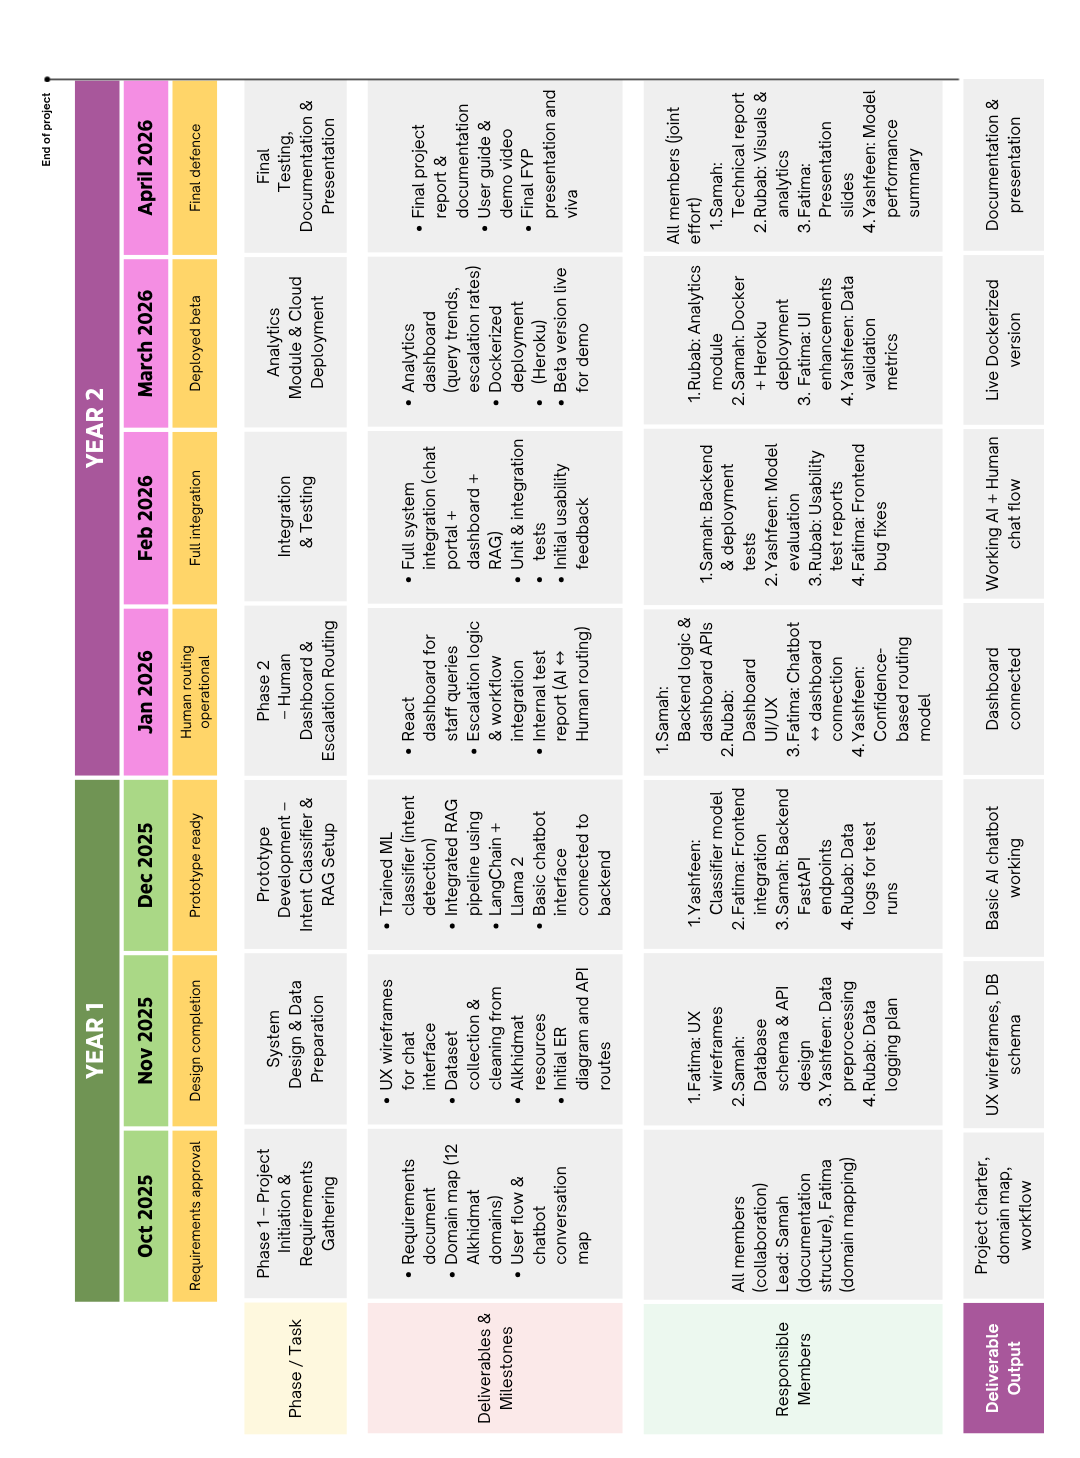
\includegraphics[width=0.8\textwidth]{chapters/GanttChart.png}
    \caption{Month-Wise Deliverables}
    \label{fig:Gantt Chart}
\end{figure}

\subsection*{Deliverables Overview}
The Gantt chart above outlines the project objectives, key milestones, and timelines for each phase across Kaavish~I and Kaavish~II. Major deliverables include:
\begin{itemize}
    \item \textbf{Kaavish I:} System requirements analysis, dataset design, RAG knowledge base creation, chatbot workflow design, and prototype implementation of the frontend and backend communication pipeline.
    \item \textbf{Kaavish II:} Integration of AI/ML modules (intent classification, multimodal processing), deployment on cloud infrastructure (Heroku/Docker), human escalation dashboard, and final evaluation with Alkhidmat’s stakeholders.
\end{itemize}

\subsection*{Resources Needed}
While the Gantt chart defines tasks, timelines, and team responsibilities, successful execution also depends on the following essential resources:

\begin{enumerate}
    \item \textbf{Hardware and Computing Resources}
    \begin{itemize}
        \item Developer laptops with minimum 16GB RAM and GPU support for model inference.
        \item Cloud hosting credits or Heroku dynos for deployment and load testing.
        \item External SSDs for backup of datasets and logs.
    \end{itemize}

    \item \textbf{Software and Development Tools}
    \begin{itemize}
        \item \textbf{Backend:} FastAPI, Python, LangChain, and Llama~2 integration.
        \item \textbf{Frontend:} React.js, Tailwind CSS, and WhatsApp Business API integration.
        \item \textbf{Database and Storage:} PostgreSQL, Elasticsearch, and Firebase (for chat logs and persona data).
        \item \textbf{Version Control and CI/CD:} GitHub, Docker, and Heroku pipelines.
    \end{itemize}

    \item \textbf{AI/ML and Data Resources}
    \begin{itemize}
        \item Access to pretrained LLMs (e.g., Llama~2 or OpenAI API for evaluation).
        \item Dataset curation support from Alkhidmat domain experts for healthcare, donation, and welfare programs.
        \item Preprocessing tools for Roman Urdu and Urdu text normalization.
    \end{itemize}

    \item \textbf{Human Resources}
    \begin{itemize}
        \item \textbf{Development Team:} 4 members (Frontend, Backend, NLP, and Integration roles).
        \item \textbf{Supervisors:} Internal advisor for technical oversight; external industry mentor from Alkhidmat.
        \item \textbf{Domain Experts:} Staff providing verified data and validating chatbot responses.
        \item \textbf{Test Users:} Donors, patients, and volunteers for pilot testing and feedback collection.
    \end{itemize}

    \item \textbf{Other Resources}
    \begin{itemize}
        \item Secure API keys for WhatsApp Business and cloud hosting.
        \item Access to Alkhidmat’s internal documentation, SOPs, and donation workflow data.
        \item Dataset annotation tools for custom tagging of healthcare and donation intents.
    \end{itemize}
\end{enumerate}

\noindent
These resources collectively ensure that each phase of development outlined in the Gantt chart is feasible and aligned with the technical and operational goals of the project.

\section{Key Challenges}

This section mentions the key challenges that we foresee in this project and possible ways to address them.
\begin{enumerate}
    \item \textbf{Data Acquisition and Knowledge Base Consolidation (Pre-deployment)}
    \begin{itemize}
        \item \textbf{Challenge:} Acquiring data and building a reliable RAG knowledge base is an immediate challenge since Al-Khidmat does not currently have a single, consolidated, structured database. This requires extensive web scraping and manual formatting of disparate documents across multiple domains, which is complicated by time constraints and the need for domain expertise.
        \item \textbf{Mitigation:} This challenge has been explicitly communicated to the external supervisor. The team has prioritized the most impactful datasets through user personas (e.g., Blood Donation SOPs). The mitigation strategy involves assigning a dedicated industry partner resource to gather and provide this essential, formatted data ASAP, aiming for the core datasets to be compiled within the next 1--2 weeks.
    \end{itemize}
    \item \textbf{Multilingual and Roman Urdu Accuracy (Natural Language Processing)}
    \begin{itemize}
        \item \textbf{Challenge:} Achieving high accuracy in Urdu and handling the inconsistency of Roman Urdu (Urdu written in English script) is difficult, as LLMs often lack high fidelity for low-resource languages and phonetic variations. This directly impacts the $\geq 90\%$ accuracy goal.
        \item \textbf{Mitigation:} Dedicate significant effort to curating the Urdu component of the RAG knowledge base. Employ custom preprocessing steps to normalize common Roman Urdu spellings before feeding them to the LLM/RAG engine.
    \end{itemize}

    \item \textbf{RAG Data Volatility and Latency (Data Management)}
    \begin{itemize}
        \item \textbf{Challenge:} Al-Khidmat's program details (e.g., active disaster relief efforts, current blood stock) change frequently. Since the system relies on a \textbf{periodically updated} knowledge base, there is a risk of providing outdated information, which compromises user trust and data integrity.
        \item \textbf{Mitigation:} Establish clear and enforced SLA for Admin updates to the RAG knowledge base (e.g., daily update requirement for time-sensitive domains like Blood Services). Use the Human Escalation Dashboard to flag and correct critical data mismatches immediately.
    \end{itemize}

    \item \textbf{Balancing Transparency and Privacy (Security and Ethics)}
    \begin{itemize}
        \item \textbf{Challenge:} Donors seek transparency about fund utilization, but the system must rigorously protect beneficiary and personal data (e.g., Zakat recipient details, patient health information) while maintaining local compliance standards.
        \item \textbf{Mitigation:} Implement stringent anonymization/pseudonymization for all data logs. Use guardrails to strictly prevent the LLM from generating or retrieving specific identifiable information in public responses.
    \end{itemize}

    \item \textbf{Human Handoff and Agent Training (Operational/UX)}
    \begin{itemize}
        \item \textbf{Challenge:} Ensuring a seamless handover from AI to a human agent without frustrating the user, particularly on WhatsApp where the 24-hour window constraint applies. Agents also need specialized training to use the Human Escalation Dashboard efficiently (diagnosing the bot's failure, not just the user's query).
        \item \textbf{Mitigation:} Focus on quick context loading and pre-filled response templates in the dashboard. Develop mandatory training modules for agents specifically on "AI Failure Diagnosis" and persona-aware communication.
    \end{itemize}
\end{enumerate}

\chapter{Literature Review}
\label{chap:lit}
% This chapter presents the current state of the art in the domain and talks about other similar work that has been done in this area. It also establishes the novelty of our work by highlighting the differences between the existing work and our work.

% We will keep updating this chapter (especially if our project is research-intensive) as our research proceeds and we come across more work related to our problem.

% Of course, we take inspiration from \cite{einstein} but wish the work was typeset in \LaTeX \cite{knuthwebsite}, e.g. by taking help from \cite{latexcompanion}.

\section{Introduction}

The rapid advancement of artificial intelligence (AI), particularly large language models (LLMs), has significantly reshaped organizational knowledge management and service delivery. Retrieval-Augmented Generation (RAG) enhances LLMs by grounding responses in external knowledge sources, improving factual accuracy, reducing hallucinations, and increasing transparency \cite{lewis2020rag,gao2023ragsurvey,fan2024ragllm}. In parallel, nonprofit and humanitarian organizations are increasingly adopting conversational systems for service navigation, donor engagement, and community outreach \cite{folstad2018socialgood,siddiqi2024bablibot,munir2021bablibot}.

This literature review synthesizes research across four interconnected areas to inform the design of a multi-domain organizational assistant for a Pakistani NGO. First, it examines RAG-based conversational systems, including advances in persona adaptation, multi-turn dialogue, and multimodal interaction. Second, it reviews chatbot deployments for social good, with a focus on low- and middle-income country (LMIC) contexts and local-language systems in Urdu and Roman Urdu. Third, it explores system-level considerations, including human-in-the-loop escalation, operational dashboards, and analytics. Finally, it considers infrastructure, security, and deployment practices required for scalable and reliable systems.

A key gap emerges from this synthesis: existing chatbot systems in Pakistan are predominantly single-domain and loosely integrated with organizational workflows. There is limited evidence of a unified, multi-domain RAG-based assistant capable of supporting donations, healthcare services, blood programs, and welfare initiatives across English, Urdu, and Roman Urdu. The proposed Alkhidmat Public Chat Portal addresses this gap by combining RAG grounding, multilingual interaction, multimodal inputs, confidence-aware escalation, and integrated operational tooling within a single system.

\section{State of the Art in RAG-Based Organizational Assistants}
For tasks that require a lot of knowledge, Retrieval-Augmented Generation (RAG) was introduced as a general framework that combines pretrained sequence to sequence models with a non-parametric memory of retrieved documents \cite{lewis2020rag}. Lewis et al. note that models augmented with retrieval not only generate more accurate and factual responses but also outperform both purely parametric models and traditional retrieve-and-extract approaches in open-domain question answering.

The RAG framework has since been organised and made clearer by a number of survey studies.  A thorough analysis of RAG in large language models is given by Gao et al. \cite{gao2023ragsurvey}, who also discuss naive, advanced, and modular architectures and explain how the retrieval, generation, and augmentation components interact.  Similar to this, Fan et al. concentrate on Retrieval-Augmented Large Language Models (RA-LLMs), looking at their architectures, training methods, and uses in domains like recommendation systems and customer service \cite{fan2024ragllm}.  When taken as a whole, these surveys show that RAG has emerged as a crucial strategy for producing organisational assistants who are trustworthy and able to maintain a solid foundation in current, authoritative knowledge.

At the same time, research on conversational AI has made significant progress in areas such as persona modeling, multi-turn context tracking, and socially aware interactions. Surveys of neural conversational agents show a clear shift from simple, single-turn question answering toward multi-turn, task-oriented, and open-domain dialogue systems that can adapt both style and content to meet users’ needs \cite{kim2023convai}. Persona-aware dialogue models take this a step further, adjusting tone and content based on user or role profiles—an important consideration when designing assistants for beneficiaries, donors, or staff who may have different information requirements \cite{singh2024persona}.

From these trends, contemporary organizational assistants typically:
\begin{itemize}\setlength{\itemsep}{0pt}
    \item use RAG to ground answers in internal knowledge bases;
    \item support multi-channel access (web, mobile, messaging apps);
    \item adapt to different user personas and roles;
    \item include monitoring, guardrails, and human-in-the-loop escalation.
\end{itemize}
The proposed Alkhidmat assistant follows this pattern by coupling an LLM front-end with domain-structured knowledge on donations, healthcare, blood services, and welfare programmes, plus escalation and analytics for staff.

\section{AI Chatbots in Nonprofits and Civil Society}
While RAG provides the technical foundation for knowledge-grounded systems, its application in real-world settings—particularly in the nonprofit sector—introduces additional design constraints related to accessibility, trust, and inclusion. 

Within the nonprofit and social-impact space, there is growing interest in deploying chatbots for information provision, advocacy and service navigation. Følstad et al.\ discuss “chatbots for social good’’ as a research and design agenda, identifying use cases in health, education, civic participation and humanitarian response, and highlighting issues of inclusion, trust, and governance \cite{folstad2018socialgood}. They note that many early systems are narrowly scoped, relying on scripted or intent-based flows.

Empirical work on health-related chatbots in low and middle income countries (LMICs) provides concrete examples. Munir et al.\ report on the feasibility of an “artificially intelligent vaccines chatbot’’ (Bablibot) in Pakistan, deployed via text messaging to provide immunization information to caregivers in low-income communities \cite{munir2021bablibot}. Their mixed-methods evaluation finds high user satisfaction and suggests that chatbots can address access barriers, especially for women. Building on this, Siddiqi et al.\ present a detailed mixed-methods study of Bablibot, describing its design using natural language processing (NLP), machine learning and a human-in-the-loop component, and show that local-language chatbots are feasible and acceptable in low-resource, low-literacy settings \cite{siddiqi2024bablibot}.

Beyond health, chatbots are increasingly used for fundraising and advocacy by nonprofit organizations, including for storytelling and campaign communication on platforms such as Facebook Messenger \cite{halperin2023storytelling}. However, many of these systems focus on a single function (e.g., advocacy narratives, fundraising journeys) and are not deeply integrated with internal programme databases or multi-department service structures.

\section{Pakistan Context and Local-Language Chatbots}
These challenges are further amplified in the Pakistani context, where linguistic diversity and resource constraints shape the design and deployment of conversational systems. Pakistan is an important context for AI-mediated services because it is a lower middle income, linguistically diverse country with high mobile and messaging usage.  Rich morphology, complex script, and cross-script usage are some of the unique NLP challenges faced by Urdu and Roman Urdu.  In their review of problems and difficulties in Urdu Natural Language Processing, Khan et al. point out the lack of annotated tools and resources and identify tasks like tokenisation, morphological analysis, POS tagging, parsing, and named-entity recognition as ongoing research issues \cite{khan2020urdunlp}.  The development of Urdu NLP resources and applications is also described in a more comprehensive survey of Urdu language processing \cite{anwar2016survey}.

Several recent projects have focused on Urdu and Roman Urdu in conversational AI. For instance, Kumar et al. developed SAATHI, a voice-enabled Urdu virtual assistant designed to help senior citizens in Pakistan who are “ageing in place” by providing news, reminders, and simple interactions in Urdu \cite{kumar2022saathi}. In another project, Mohiuddin et al. created a multilingual Urdu chatbot using the Rasa framework, which tackles the challenge of converting Roman Urdu input into Urdu intents \cite{mohiuddin2023multilingual}. Similarly, Hakeem et al. describe an AI-powered chatbot for Roman Urdu, combining GPT-style models with a RAG framework to improve handling of spelling variations and the lack of standardization \cite{hakeem2025romanurdu}.

At the same time, evaluation of LLMs on Urdu remains an active area. Kazi et al.\ evaluate large language models on Urdu–English question answering, showing significant performance gaps between high-resource and low-resource settings and underlining the need for Urdu-specific adaptation and datasets \cite{kazi2025llmqa}. These works collectively demonstrate that:
\begin{itemize}\setlength{\itemsep}{0pt}
    \item Urdu and Roman Urdu chatbots are technically feasible;
    \item local-language assistants can be deployed in low-resource Pakistani communities;
    \item there is still limited work on large, multi-domain assistants tightly integrated with a single NGO’s internal systems.
\end{itemize}

\section{Similar Work in NGO Service and Donor Assistants}
Building on these contextual considerations, prior work on NGO-oriented assistants can be grouped into distinct categories based on domain scope and system capabilities. In the specific domain of nonprofit and NGO assistants, the most relevant academic work can be grouped into three strands.

First, chatbots for social good and humanitarian applications. The CHI extended abstract on chatbots for social good explicitly frames chatbots as tools for health, education and civic engagement, and calls for systems that can scale while remaining inclusive and trustworthy \cite{folstad2018socialgood}. This provides a conceptual foundation for NGO-oriented assistants such as the Alkhidmat portal.

Second, health and immunization chatbots in Pakistan. Munir et al.\ and Siddiqi et al.\ both focus on Bablibot, a local-language chatbot for immunization information in Karachi \cite{munir2021bablibot,siddiqi2024bablibot}. Bablibot is tightly connected to immunization registries and demonstrates integration with digital health records, but it is single-domain (vaccines) and not a general NGO service portal.

Third, Urdu / Roman Urdu service chatbots and administrative bots. Mohiuddin et al.\ target multi-lingual service access via transliteration-based Urdu chatbots using Rasa \cite{mohiuddin2023multilingual}; Kumar et al.\ design SAATHI for elderly care information \cite{kumar2022saathi}; Hakeem et al.\ build a Roman Urdu chatbot using RAG for more open-ended conversational understanding \cite{hakeem2025romanurdu}. Maqbool et al.\ propose a sentence-level encoder–decoder architecture for an intelligent administrative chatbot for Roman Urdu, designed to support university administrative tasks \cite{maqbool2025adminbot}. These systems are structurally closer to an organizational assistant, but they are focused on administrative or general chat tasks rather than multi-department NGO services.

There is little evidence in the academic literature of a \emph{single} Pakistani NGO deploying a RAG-based assistant that simultaneously covers donations, healthcare navigation, blood services, welfare programmes, and volunteer opportunities across web and WhatsApp.

\section{Multimodal Inputs and Accessibility} 
Modern conversational assistants increasingly handle not just text but multiple input modalities, such as images and voice, significantly enhancing accessibility and interaction.

Recent work on Multimodal RAG (Retrieval-Augmented Generation) shows how chatbots can analyze and reason over images, tables, and text together to enrich responses. For instance, systems can perform OCR or caption images and retrieve relevant text or table data to answer user queries, reflecting an alignment with research on "multimodal" chatbots that combine vision and language for richer dialogue \cite{gulab2024multimodalrag}.

State-of-the-art models, such as GPT-4V ("GPT-4 with Vision"), now support direct image input, processing raw image bytes alongside text \cite{gulab2024multimodalrag}. OpenAI has added similar image and voice capabilities to ChatGPT, allowing users to "show ChatGPT what you’re talking about" and converse by voice \cite{openai2023multimodal}. An AI chatbot might use convolutional neural networks (CNNs) to parse objects and context from an uploaded photo \cite{ijaresm2024multimodal}.

In practical terms, this means our chatbot can accept photos of payment receipts, prescriptions, or donation screenshots and extract contextual information from them \cite{gulab2024multimodalrag}.

Voice interfaces are also becoming common for accessibility:
\begin{itemize}\setlength{\itemsep}{0pt}
    \item A speech-to-text (STT) or automatic speech recognition (ASR) component can transcribe user voice notes (with basic Urdu support) into the dialogue, allowing users who prefer speaking to interact with the bot  \cite{gulab2024multimodalrag}, \cite{ijaresm2024multimodal}.
    \item In a Pakistani NGO context, this means a donor could send a voice note in Urdu that is transcribed and answered via ASR, bridging literacy and connectivity gaps \cite{ijaresm2024multimodal}, \cite{openai2023multimodal}.
\end{itemize}

Integrating image and speech inputs enables the system to serve non-tech-savvy, low-literacy users, or those with disabilities, extending the chatbot beyond "plain text" to richer multimodal engagement \cite{gulab2024multimodalrag}. Such features make digital assistants more inclusive (e.g., by letting low-literacy users show receipts or speak questions) \cite{openai2023multimodal}.

These multimodal capabilities are rapidly dropping in cost and complexity as open-source vision models (e.g., CLIP, BLIP-2) and multimodal LLM APIs (e.g., GPT-4V, Claude Vision) become more accessible \cite{gulab2024multimodalrag}.

\section{Human-in-the-Loop and Escalation Management}
Industry best practices emphasize that chatbots should gracefully escalate complex or ambiguous queries to human agents to maintain user trust and ensure effectiveness \cite{freshworks2024analytics}. In hybrid AI support systems, escalation is typically triggered when the model’s confidence is low or when the user’s request falls outside the chatbot’s defined domain, such as medical emergencies or detailed calculations. These systems rely on monitoring intent confidence and transferring any ambiguous or sensitive query to staff to prevent misinformation and ensure reliability \cite{freshworks2024analytics}. Platforms such as WATI, a WhatsApp Business API provider, operationalize this principle by implementing hybrid workflows in which the AI bot “automatically answers common queries” but “routes more complex queries to your support teams/agents based on customer intent” \cite{wati2024aisupport}. In addition, industry vendors stress that human agents must retain complete control to manage AI conversations manually when required, ensuring operational oversight, accountability, and continuity in user experience.

\subsection{Uncertainty Estimation and Confidence Scoring in RAG Systems}
A key challenge in implementing human-in-the-loop systems is determining \emph{when} escalation should occur. This requires explicit estimation of model confidence and uncertainty, which has become an active area of research in LLM-based systems. Reliable deployment of RAG-based assistants requires explicit modeling of uncertainty to decide when to answer, abstain, or escalate. Recent work categorizes confidence estimation methods into four classes: token-level, self-verbalized, semantic similarity-based, and mechanistic approaches \cite{acm2024uncertainty}.

\textbf{Token-level methods} leverage the probabilistic nature of LLMs. Since models generate tokens sequentially with associated probabilities, confidence can be derived from log-probabilities. Common techniques include:
\begin{itemize}\setlength{\itemsep}{0pt}
    \item \textit{Average log-probability} and \textit{maximum token uncertainty} for sequence-level confidence;
    \item \textit{Perplexity}, where higher values indicate greater uncertainty due to a flatter probability distribution;
    \item \textit{Entropy-based scoring}, where low entropy reflects confident (peaked) token distributions and high entropy indicates uncertainty \cite{acm2024uncertainty}.
\end{itemize}

Recent applied approaches propose weighted confidence formulations that emphasize high-certainty tokens. For example, combining the joint probability of top-ranked tokens with overall sequence probability (e.g., 70/30 weighting) has been shown to stabilize confidence estimates in generation tasks \cite{thomas2024confidence}.

\textbf{Sampling-based methods}, such as SelfCheckGPT, estimate confidence by generating multiple responses and measuring consistency across them. Higher agreement across sampled outputs implies higher confidence, making this approach suitable for black-box models where logits are unavailable, albeit at higher computational cost \cite{capgemini2024uncertainty}.

\textbf{Self-verbalized confidence} asks the model to report its own certainty. While simple, this approach is prone to overconfidence and is typically used in combination with other signals \cite{capgemini2024uncertainty}.

\textbf{Retrieval-aware confidence} is also critical in RAG systems. A common proxy is the semantic similarity between the query and retrieved documents (e.g., cosine similarity), aggregated across top-$k$ chunks to estimate retrieval reliability \cite{geeksforgeeks2024ragmetrics}. This complements generation-side confidence.

\textbf{Threshold selection} plays a central role in operationalizing confidence. Industry and research suggest tuning thresholds empirically on validation data to optimize correctness, often by sweeping values between 0 and 1 and selecting those that maximize accuracy for high-confidence responses \cite{mit2022overconfidence,cyara2023threshold}. These thresholds directly inform fallback strategies such as abstention or human escalation.

\textbf{Implication for system design:} In the proposed system, confidence is modeled as a hybrid signal combining (i) token-level generation confidence, (ii) retrieval similarity scores, and (iii) optional sampling-based validation for critical queries. This composite score governs response acceptance, rejection (“I don’t have enough information”), and routing to human agents, aligning with best practices for trustworthy AI deployment.


\section{Staff Coordination and Agent Dashboard}
The operationalization of human-in-the-loop handoff is facilitated through shared agent dashboards, often referred to as “team inboxes,” as exemplified by platforms such as WATI \cite{wati2024aisupport}. These dashboards are designed to enable seamless coordination among staff when managing escalated queries. Each escalated chat is presented as a ticket, allowing agents to access the complete conversation history and respond directly through the same channel, including bilingual responses where required \cite{wati2024aisupport}. Domain-based routing capabilities are commonly integrated, ensuring that specific queries, such as those related to donations, are directed to the appropriate team (e.g., fundraising) and can be dynamically reassigned among specialists. The inclusion of pre-approved templates supports standardized and high-quality responses, particularly within platform-specific constraints such as WhatsApp’s 24-hour reply window, while the logging of agent actions provides traceability and auditability. Furthermore, these systems are designed to maintain continuous availability and multilingual support, enabling consistent handoff and follow-up interactions irrespective of whether the user communicates in English, Urdu, or Roman Urdu. Vendors highlight that such implementations provide “24/7 automated support that responds naturally and accurately in your customers’ preferred language” \cite{wati2024aisupport}, thereby ensuring both operational efficiency and user satisfaction.

\section{Analytics and Admin Tools}
Effective deployments of organizational chatbots require comprehensive analytics and content management to guide continuous improvement, maintain accuracy, and ensure transparency over time. Performance monitoring is typically conducted through analytics dashboards that report Key Performance Indicators (KPIs) such as query volume, total queries handled, and deflection rate, indicating the percentage of interactions resolved by the AI versus those escalated to human agents. Industry guides emphasize escalation or human-takeover rate as a vital KPI, noting that low takeover rates suggest strong autonomous handling, whereas spikes may signal knowledge gaps or safety concerns \cite{freshworks2024analytics}. Additional time-based metrics commonly tracked include average response time and session duration, and systems routinely collect user satisfaction data, including CSAT (thumbs-up/down), to assess perceived quality \cite{freshworks2024analytics}. Real-time dashboards also chart usage by domain (e.g., donations or health queries) and peak hours, enabling administrators to interpret logs, review conversation transcripts, and incorporate user feedback to iteratively improve the bot, refine intents or flows, and update the RAG knowledge base \cite{freshworks2024analytics}. The literature consistently underscores that chatbots must function as “data-driven” tools \cite{freshworks2024analytics}.

A human-facing administrative interface complements analytics by enabling operational control and content management. Staff require the ability to manually update program information, such as donation campaigns and hospital details, and maintain the knowledge repository. In the context of a Pakistani NGO, such an interface would also allow editing of Urdu translations, defining personas, and monitoring escalation tickets in real time. Administrative configuration capabilities typically include adjusting fallback messages, modifying quick-reply templates, and setting content moderation rules. Systems comparable to enterprise chat platforms incorporate “team inbox” operational views alongside update forms for knowledge base maintenance \cite{wati2024aisupport}. Together, automated analytics and manual administrative controls align with recognized best practices in RAG-based assistant deployment, ensuring sustained accuracy, transparency, and ongoing system improvement.

\section{Cloud Deployment and Scalability}
To accommodate large user volumes, ensure high availability, and facilitate rapid growth, conversational platforms are typically deployed on cloud infrastructure with containerized architectures. Many organizations, including non-governmental organizations (NGOs), leverage Platform-as-a-Service (PaaS) solutions such as Heroku, AWS, and Google Cloud, which provide autoscaling capabilities, managed databases, and high availability \cite{heroku2024chatbots}, \cite{aws2024marketplace}. Salesforce’s Live Agent chatbot, for instance, is deployed on Heroku, utilizing managed Postgres databases and benefiting from dedicated operational staff responsible for backups, updates, and outage management, thereby reducing the operational burden on developers \cite{heroku2024chatbots}. Heroku advertises its PaaS offering as providing “fully managed infrastructure... with built-in autoscaling and detailed performance metrics” in a “compliant environment.”  

The use of PaaS or containerized cloud clusters ensures both high availability and seamless horizontal scalability, enabling the system to accommodate hundreds of simultaneous users and remain resilient during peak usage periods \cite{heroku2024chatbots}. Managed cloud services further enhance operational efficiency by providing automated backups, secure key management, and CI/CD pipelines for version control, along with real-time performance monitoring \cite{heroku2024chatbots}, \cite{aws2024marketplace}. Technical components of such deployments often include Docker containers, and services like Elasticsearch or pgvector for Retrieval-Augmented Generation (RAG) indexing, which support maintainable and responsive chatbot systems. Leveraging these cloud-based practices enables platforms to reliably support large-scale user interactions while maintaining uptime exceeding 99\%.

\section{Security, Privacy, and Compliance}
For NGOs deploying conversational agents, safeguarding user data is of paramount importance and must align with both industry standards and relevant legal frameworks. The architecture of such systems should integrate robust encryption mechanisms, ensuring that all communications, particularly those containing sensitive personal or medical information, are secured in transit and at rest. For web interactions, HTTPS/TLS protocols should be applied, while WhatsApp-based interactions benefit from end-to-end Signal encryption inherent to the platform \cite{whatsapp2024trust}.  

Beyond technical security, adherence to global compliance standards is critical. The WhatsApp Business Platform holds certifications including SOC 2 and explicitly supports GDPR compliance, providing a framework for lawful data processing \cite{whatsapp2024trust}. In addition, organizations operating in Pakistan should comply with emerging national regulations, such as the draft Personal Data Protection Bill (2023), which mirrors GDPR by mandating user consent, data minimization, and breach accountability \cite{chambers2025pakistan}.  

Data minimization policies are central to ethical and legal compliance. Best practices include obtaining explicit user consent \cite{whatsapp2024trust}, \cite{chambers2025pakistan}, retaining only transient session logs, and deleting chat histories after completion of interactions \cite{whatsapp2024trust}. Personal identifiers should be anonymized, and sensitive personally identifiable information (PII) should not be stored beyond operational necessity \cite{chambers2025pakistan}.  

In conclusion, a secure and compliant chatbot deployment integrates the built-in end-to-end encryption and certifications of the WhatsApp Business API while implementing internal policies for data minimization and local regulatory compliance. This combination ensures both technical security and adherence to legal and ethical standards, providing a reliable framework for NGO services \cite{whatsapp2024trust}, \cite{chambers2025pakistan}.

\section{Differences Between Existing Work and the Proposed System}
Synthesizing the above, the proposed Public Chat Portal for Alkhidmat differs from existing work in several ways.

\subsection{Multi-Domain NGO Scope Versus Single-Domain Chatbots}
Existing Pakistani chatbots in the literature typically focus on one domain: immunization (Bablibot) \cite{munir2021bablibot,siddiqi2024bablibot}, elderly care information (SAATHI) \cite{kumar2022saathi}, administrative tasks in education \cite{maqbool2025adminbot}, or general Roman Urdu conversational understanding \cite{hakeem2025romanurdu}. In contrast, the Alkhidmat assistant is explicitly designed as a multi-department organizational portal, covering donations (e.g., Zakat, Sadaqah), healthcare facilities, blood services (donation and requests), other general facilities.

\subsection{Deep RAG Over NGO-Specific Knowledge}
Most NGO-relevant chatbots described in the literature are intent or flow based, with relatively shallow use of organizational documents or databases \cite{folstad2018socialgood,mohiuddin2023multilingual}. By contrast, the proposed system follows the RAG paradigm discussed by Lewis et al.\ and later surveys \cite{lewis2020rag,gao2023ragsurvey,fan2024ragllm}, building a structured knowledge base from Alkhidmat’s internal SOPs, programme descriptions, facility lists, and operational data, and using retrieval to ground responses. This is closer to enterprise RAG assistants but applied in a nonprofit setting.

\subsection{Localization to Urdu, Roman Urdu, and Pakistani NGO Practices}
While prior work has shown that Urdu and Roman Urdu chatbots are feasible \cite{khan2020urdunlp,kumar2022saathi,mohiuddin2023multilingual,hakeem2025romanurdu}, these systems are typically either domain-specific (health, elderly care) or experimental. The Alkhidmat assistant aims to:
\begin{itemize}\setlength{\itemsep}{0pt}
    \item support English, Urdu, and basic Roman Urdu input;
    \item incorporate programme names and concepts specific to a large Pakistani NGO (e.g., Mawakhat, Orphan Care, Bano Qabil);
    \item operate on channels (web and WhatsApp Business) that match actual user behaviour in Pakistan.
\end{itemize}
This combination of linguistic and institutional localization is not extensively covered in existing academic work.

\subsection{Integration With Operational Systems and Human Escalation}
The Bablibot work demonstrates integration with immunization registries and a human-in-the-loop support model \cite{siddiqi2024bablibot,munir2021bablibot}. The proposed Alkhidmat portal extends this logic beyond health to other NGO operations, for example:
\begin{itemize}\setlength{\itemsep}{0pt}
    \item a blood-donation microservice that can check donor eligibility criteria and facility locations;
    \item dashboards where staff can view escalated conversations with context and respond directly;
    \item analytics on domain-wise query volumes, response quality, and escalation rates.
\end{itemize}
This reflects best practices in RAG-based enterprise assistants (monitoring, feedback loops) but adapted for NGO governance.
Escalation decisions are typically driven by confidence thresholds derived from uncertainty estimation. Queries with low generation confidence or weak retrieval grounding are automatically routed to human agents, ensuring reliability and preventing hallucinated responses \cite{mit2022overconfidence,cyara2023threshold}.

\section{Conclusion}
The literature establishes Retrieval-Augmented Generation as a robust framework for building grounded and reliable conversational systems. At the same time, research in conversational AI emphasizes the importance of multi-turn interaction, persona adaptation, and user trust. In nonprofit contexts, chatbot deployments demonstrate feasibility and impact, particularly in LMIC settings, but remain largely narrow in scope and function.

\chapter{Software Requirement Specification (SRS)}
\label{chap:srs}
This chapter provides detailed specifications of the system under development.

\section{Functional Requirements}

% This section describes each function/feature provided by our system. These functions are logically grouped into modules based on their purpose/users/mode of operations etc (as per our system). A functional hierarchy may look like:
Functional requirements are grouped into modules corresponding to major system components. 
\begin{outline}
  \1 Core Chatbot Module (Public Facing)
  \2 Multimodal Input Handling
  \3 Text Input: Accept text queries in English, Urdu, and Roman Urdu (basic level).
  \3 Image Input: Analyze uploaded images for contextual information (e.g., payment receipts, prescriptions, donation screenshots). Handwritten text recognition is out of scope for MVP. 
  \3 Voice Input (Phase 2 - Conditional): Convert voice messages to text using Speech-to-Text API. Basic Urdu support only; dialect variations are out of scope. Voice integration depends on successful testing of Phase 1 text-based system. 
  \4 \textit{MVP Scope: Phase 1 focuses on duo-lingual text (English + Urdu) and image input only.}
  \2 Intent Classification \& Domain Identification 
  \3 Domain Classification: Automatically identify the query domain from four categories:  
  \4 Donation: Payment methods, project details, Zakat/Sadaqah eligibility 
  \4 Healthcare: Hospital locations, services, appointments, ambulances 
  \4 Blood Services: Donor eligibility, blood bank locations, blood group availability 
  \4 General Inquiry: Organization information, volunteering, events, queries about other domains
  \4 \textit{Note: this does not cover the exhaustive list of data for the domains mentioned}
  \3 Intent Clarification Loop: When queries are ambiguous or confidence score is low, prompt user with clarifying questions before proceeding (e.g., "Are you asking about blood donation or healthcare services?"). 
  \3 Confidence Threshold: Queries with confidence score below 0.7 are flagged for human escalation. 
  \2 Contextual Response Generation 
  \3 RAG-Based Retrieval: Retrieve verified information from the domain-structured knowledge base using Retrieval-Augmented Generation. 
  \3 Persona-Aware Responses: Adapt response length, tone, and detail based on identified user persona (e.g., overseas donor, non-tech-savvy patient, recurring donor). 
  \3 Follow-Up Context: Maintain session context to handle follow-up questions that depend on prior conversation history. 
  \3 Session Management: Preserve conversation context throughout the user session to enable multi-turn dialogues.
  \2 Multilingual Response \& Accessibility 
  \3 Language Selection: Allow users to select their preferred language (English or Urdu) at the start of interaction. 
  \3 Quick Reply Options: Provide button-based shortcuts and pre-defined options for low-literacy users to minimize typing. 
  \3 Consistent Quality: Ensure response quality is consistent across languages with no discrepancy between English and Urdu outputs. 
  \2 Trust \& Verification
  \3 Branding Display: Show verified Alkhidmat branding, official logos, and chatbot verification messages to assure users of authenticity. 
  \3 Official Channel Verification: Display verified WhatsApp Business number and official website domain to prevent scam concerns. 
  \2 Guardrails \& Safety 
  \3 Content Moderation: Implement guardrails to prevent inappropriate responses or off-topic conversations. 
  \3 Privacy Protection: Ensure no personal data is retained beyond the session lifetime. 
  \3 Fallback Responses: Provide predefined safe responses when the system cannot confidently answer a query. 
  
  \1 Information Retrieval \& Data Management Module \\
  The knowledge base contains periodically updated, domain-structured information covering (note: this is not an exhaustive list of the data for each domain): 
  \2 RAG Knowledge Base (General Information) 
  \\\textit{Note: Knowledge base is NOT real-time; it is periodically updated by administrators. }
  \3 Donation Support: 
  \4 Active and verified campaign details (healthcare, education, orphan care, women empowerment, disaster relief) 
  \4 Payment methods and step-by-step guidance (Easypaisa, JazzCash, bank transfer, international cards, PayPal)
  \4 Zakat and Sadaqah eligibility criteria for different programs 
  \4 Donation workflow and confirmation processes
  \4 Transparency reports and impact summaries 
  \3 Healthcare Information: 
  \4 List of Alkhidmat hospitals, clinics, labs, and pharmacies with addresses and coordinates 
  \4 Service offerings per facility (OPD, diagnostics, pharmacy, ambulance) 
  \4 Operating hours and appointment procedures
  \4 Consultation fees, test charges, and medicine pricing
  \4 Doctor availability, specializations, and gender-specific staff information 
  \4 Emergency helpline numbers and ambulance booking procedures 
  \3 Program Information: 
  \4 Summaries of Alkhidmat's 12+ domains (education, water, orphan care, community services, disaster management)
  \4 Women-centric initiatives (Bano Qabil, maternity services, women empowerment) 
  \4 Youth and student programs 
  \4 Corporate Social Responsibility (CSR) partnership opportunities 
  \3 General Information: 
  \4 Organization history, mission, and credibility verification 
  \4 Volunteering opportunities and community event schedules
  \4 FAQs on trust, transparency, and fund utilization 
  \2 Blood Donation Microservice (Operational Data) \\
  A separate microservice containing transactional and inventory information integrates with the main system to handle blood donation queries: 
  \3 Donor Eligibility Validation: Check eligibility based on age, weight, hemoglobin levels, blood pressure, and donation intervals (WHO and Alkhidmat internal SOPs).
  \3 Blood Bank Locations: Retrieve nearest Alkhidmat-licensed blood bank addresses and contact information based on user location. 
  \3 Blood Group Availability: Query current blood stock levels and urgent blood group requirements. 
  \3 Donation Process Information: Provide step-by-step donation process details (registration, screening, donation, post-care instructions). 
  \3 Donor Network Registration: Allow users to register for SMS/WhatsApp alerts when their blood group is urgently needed. 
  \3 Post-Donation Guidelines: Provide medical instructions (hydration, rest, when to resume activities). 
  \3 Recipient Support: Guide blood recipients on required documents (CNIC, prescription), cross-match duration, reservation policies, and service charges. 
  \2 User Profiling \& Persona Management (Contextual Database) \\
  Maintain a separate database to store user information and enable personalized interactions: 
  \3 Persona Classification: Classify users into personas based on interaction patterns using a donor-beneficiary matrix:  
  \4 Donor personas: Overseas, Local, Recurring, First-Time, Corporate, Non-tech Savvy 
  \4 Healthcare personas: Rural/Urban Patient, New Patient, Non-tech Savvy Patient 
  \4 Blood service personas: New/Recurring Blood Donor, Blood Recipient 
  \3 Interaction History Tracking: Record user query patterns, preferred language, interaction frequency, and topics of interest. 
  \3 Dynamic Persona Updates: Update user persona classification after each interaction based on new behavioural data. 
  \3 Context-Aware Response Adaptation: Tailor response length, explanation depth, and recommendations based on identified persona (e.g., provide detailed explanations for first-time donors, concise responses for recurring donors).
  \3 Personalized Recommendations: Suggest relevant campaigns, services, or programs based on user history and persona. 
 
  \1 Human Agent Dashboard (Staff Facing) 
  \2 Escalation \& Routing 
  \3 Automatic Escalation: Forward queries with confidence score below 0.7 to relevant department-based chat agents.
  \3 Domain-Based Routing: Route escalated queries to specialized agents (Donation team, Healthcare team, Blood Services team, General Support). 
  \3 Sensitive Query Handling: Automatically escalate queries involving complaints, refunds, or personal grievances to human agents. 
  \2 Conversation Management
  \3 Real-Time Takeover: Allow human agents to join ongoing conversations within the same chat thread without disrupting user experience. 
  \3 24-Hour WhatsApp Window: Enable agents to respond within the 24-hour WhatsApp Business API interaction window.
  \3 Pre-Approved Templates: Provide agents with Meta-approved message templates for initiating conversations outside the 24-hour window. 
  \3 Conversation History Access: Enable agents to view full conversation context before responding. 
  \2 Knowledge Base \& Dialogue Management
  \3 Content Updates: Allow administrators to add, modify, or archive FAQs and program information in the RAG knowledge base. 
  \3 Dialogue Flow Definition: Enable admins to define and update pre-approved greeting messages, fallback responses, and guided conversation flows. 
  \3 Guardrail Configuration: Provide admin interface to set and adjust content moderation rules and response boundaries.
  \2 Role-Based Access Control 
  \3 Chat Agent Access: Grant domain-specific agents access only to queries within their department. 
  \3 Admin Privileges: Provide full system access to administrators for knowledge base management, guardrail settings, and user management. 
  \3 Audit Trail: Log all agent actions (view, respond, resolve) with timestamps for accountability. 

  \1 Analytics \& Logging Module 
  \2 Usage Tracking 
  \3 Query Metrics: Record total queries, query volume by domain, peak usage times, and average session duration. 
  \3 Response Time Monitoring: Track response time per query (target: 3-15 seconds based on complexity). 
  \3 Escalation Rate Tracking: Monitor percentage of queries escalated to human agents by domain. 
  \2 User Feedback Collection 
  \3 Post-Interaction Rating: Prompt users for thumbs-up/thumbs-down rating 15-20 minutes after their last query.
  \3 Follow-Up Query Check: Send a message asking if the user has any remaining questions before requesting feedback. 
  \3 Satisfaction Score Calculation: Aggregate user satisfaction metrics over time. 
  \2 Performance Analysis 
  \3 Answer Accuracy Monitoring: Track percentage of queries resolved by AI without escalation (target: $\geq$90\%). 
  \3 Domain Performance: Analyze which domains have highest accuracy, longest response times, or most escalations. 
  \3 Trend Identification: Highlight common query topics and identify emerging information needs that require knowledge base updates. 
  \2 Reporting \& Insights
  \3 Dashboard Visualization: Provide real-time analytics dashboard for administrators showing KPIs and trends.
  \3 Export Functionality: Generate CSV/PDF reports of usage metrics for management review. 
  \3 Anomaly Detection: Flag unusual query patterns (e.g., spam, repeated failures, sudden traffic spikes). 

  \1 Out of Scope 
  \2 Handling of regional Urdu dialects is beyond the current scope. The system is designed to support only standard Urdu syntax and semantics. 
  \2 The chatbot does not process handwritten text to extract text from images. 
  \2 Support for additional regional languages such as Punjabi, Sindhi, Pashto, or Balochi is out of scope. The MVP exclusively supports Urdu and English text input. 
  \2 The chatbot does not produce voice-based or audio-generated replies. All communication remains text-based for now. 
  \2 The LLM does not store personal data beyond basic identifiers (name, contact number, email). If such data already exists in the Alkhidmat database, it is retrieved for continuity; otherwise, the LLM treats the user as new. No long-term memory or profiling is maintained. 
  \2 Real-time data access is out of scope. The LLM retrieves information from the existing database, which requires manual updates. If the database is not updated, the system will rely on previously stored information and cannot refresh data automatically. 
  \2 Following features are out of scope as for phase 1 of development; In case of a successful phase 1 completion, these will be added to the scope. 
  \3 Bilingual speech input support for chatbot interaction, enabling automatic transcription and intent detection from spoken English or Urdu. 
  \3 Enhanced understanding and generation of Roman Urdu text for more natural and localized user communication. 
  \3 Advanced WhatsApp broadcasting and personalized campaign messaging to improve outreach effectiveness. 
    
\end{outline}

% --- The above is to be modified as per your project, e.g. a flat list if your system has limited functional requirements.

\section{Use Cases}
\begin{figure}[H]
    \centering
    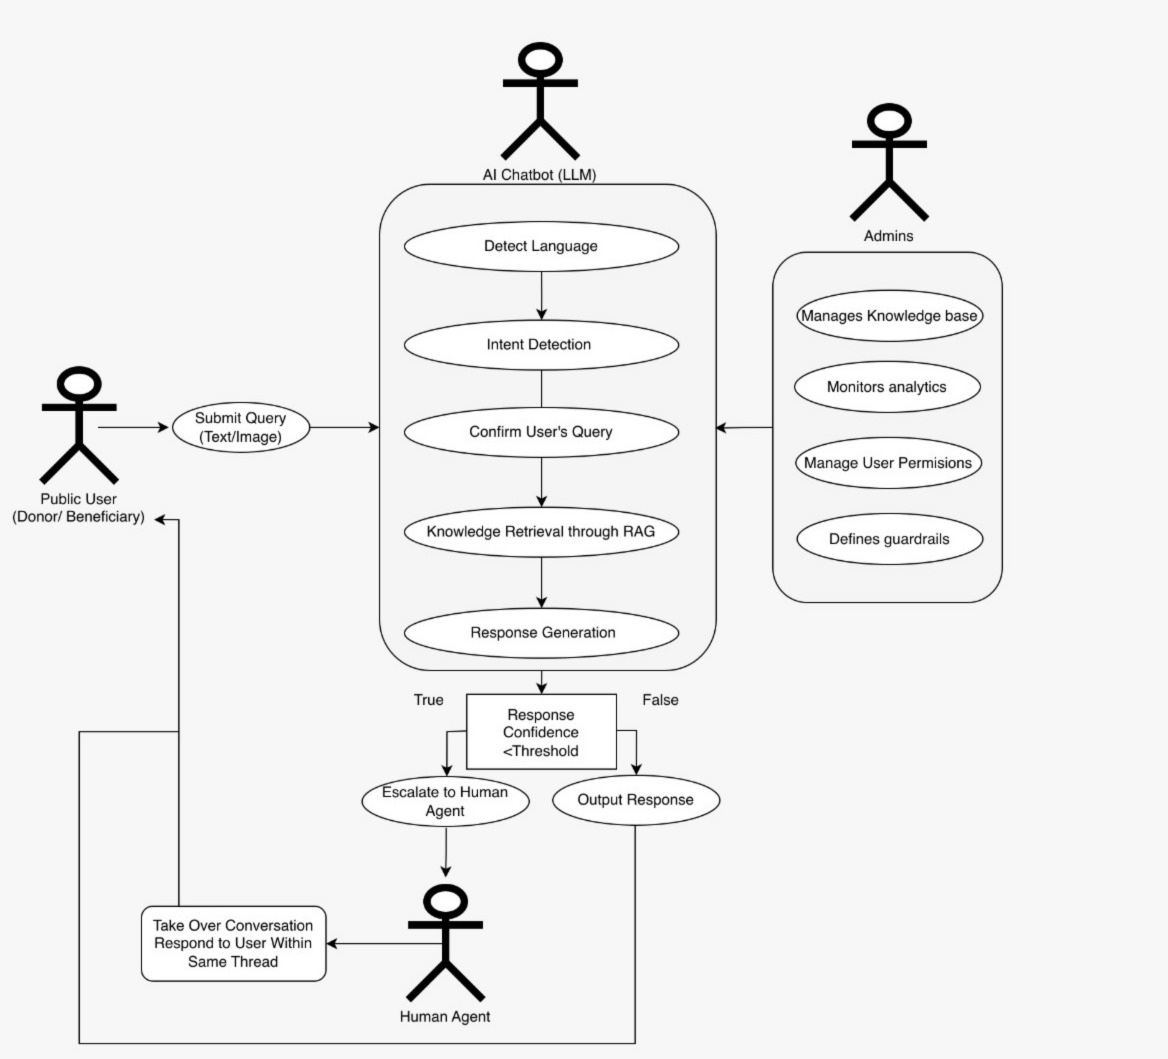
\includegraphics[width=0.9\textwidth]{chapters/srs usecase diagram.jpg}
    \caption{Use Case Diagram of the Public Chat Portal for Alkhidmat}
    \label{fig:usecase}
\end{figure}


\section{Non-functional Requirements}
\renewcommand{\arraystretch}{1.3}
\begin{longtable}{|p{3cm}|p{6.5cm}|p{6.5cm}|}
\caption{Non-Functional Requirements} \\
\hline
\textbf{Category} & \textbf{Description} & \textbf{Example} \\
\hline
\endfirsthead

\multicolumn{3}{c}%
{{\bfseries Table \thetable\ (continued): Non-Functional Requirements}} \\
\hline
\textbf{Category} & \textbf{Description} & \textbf{Example} \\
\hline
\endhead

\hline \multicolumn{3}{r}{{Continued on next page}} \\
\endfoot

\hline
\endlastfoot

\textbf{Performance} &
The system should respond within 3 to 15 seconds per query, depending on the complexity. &
Simple queries (e.g., blood bank locations) should return results in 3 seconds. Complex queries (e.g., eligibility criteria) may take up to 15 seconds. \\
\hline

\textbf{Accuracy and Relevance} &
Ensure the system provides $\geq$ 90\% accuracy and relevance in its responses to ensure reliability. &
If a user asks for blood donation instructions, the response should be factually correct and relevant in 90\% of cases. \\
\hline

\textbf{Usability / Accessibility} &
Support multilingual responses with consistent quality in both languages (e.g., English and Urdu). Include clear button-based flows for non-technical users. &
The system should provide responses in Urdu with the same clarity and accuracy as in English, without discrepancies. \\
\hline

\textbf{Reliability} &
Ensure the system maintains $>$ 90\% answer accuracy and minimal human routing. If accuracy falls below a threshold, route to a human agent. &
If a user asks for donation details and the system's confidence is below 70\%, it should route to a human agent. \\
\hline

\textbf{User Satisfaction (KPI)} &
Measure user satisfaction by asking for feedback 15--20 minutes after the last query with thumbs up/down ratings. &
After a session, if the user does not respond or replies with “no,” send a rating question (thumbs up/down) to evaluate the system's effectiveness. \\
\hline

\textbf{Data Integrity \& Backup} &
Ensure data accuracy and periodic backups of important data (e.g., RAG knowledge base). Implement automated weekly backups and data validation. &
Perform weekly automated backups of key data and ensure that data validation occurs during data entry to prevent corruption. \\
\hline

\textbf{Security / Compliance} &
Implement end-to-end encryption for all communications. Ensure no personal data retention beyond session lifetime. &
Personal data should not be retained after the session ends. The system should use encrypted communication protocols to secure sensitive information. \\
\hline

\textbf{Scalability} &
Support $\geq$ 500 simultaneous users without performance degradation using FastAPI + Elasticsearch on Docker/Heroku. &
The system should scale to support 500 simultaneous users accessing the platform without any degradation in response time. \\
\hline

\textbf{Maintainability} &
Use modular code architecture with clear documentation and API version control to ensure the system is easy to maintain and update. &
The codebase should be modular with proper documentation to allow for easy updates and troubleshooting. \\
\hline

\textbf{Compliance and Ethics} &
Adhere to Pakistan’s data privacy guidelines and AI ethics principles for NGO use. &
Ensure that the system follows local data privacy regulations and complies with ethical AI practices for non-profit organizations. \\
\hline

\end{longtable}

\section{System Diagram}
% This diagram gives a high-level view of the different components of our system and the interactions between them. Each component and the particular tools/technologies/libraries used to build it are described.
\begin{figure}[H]
    \centering
    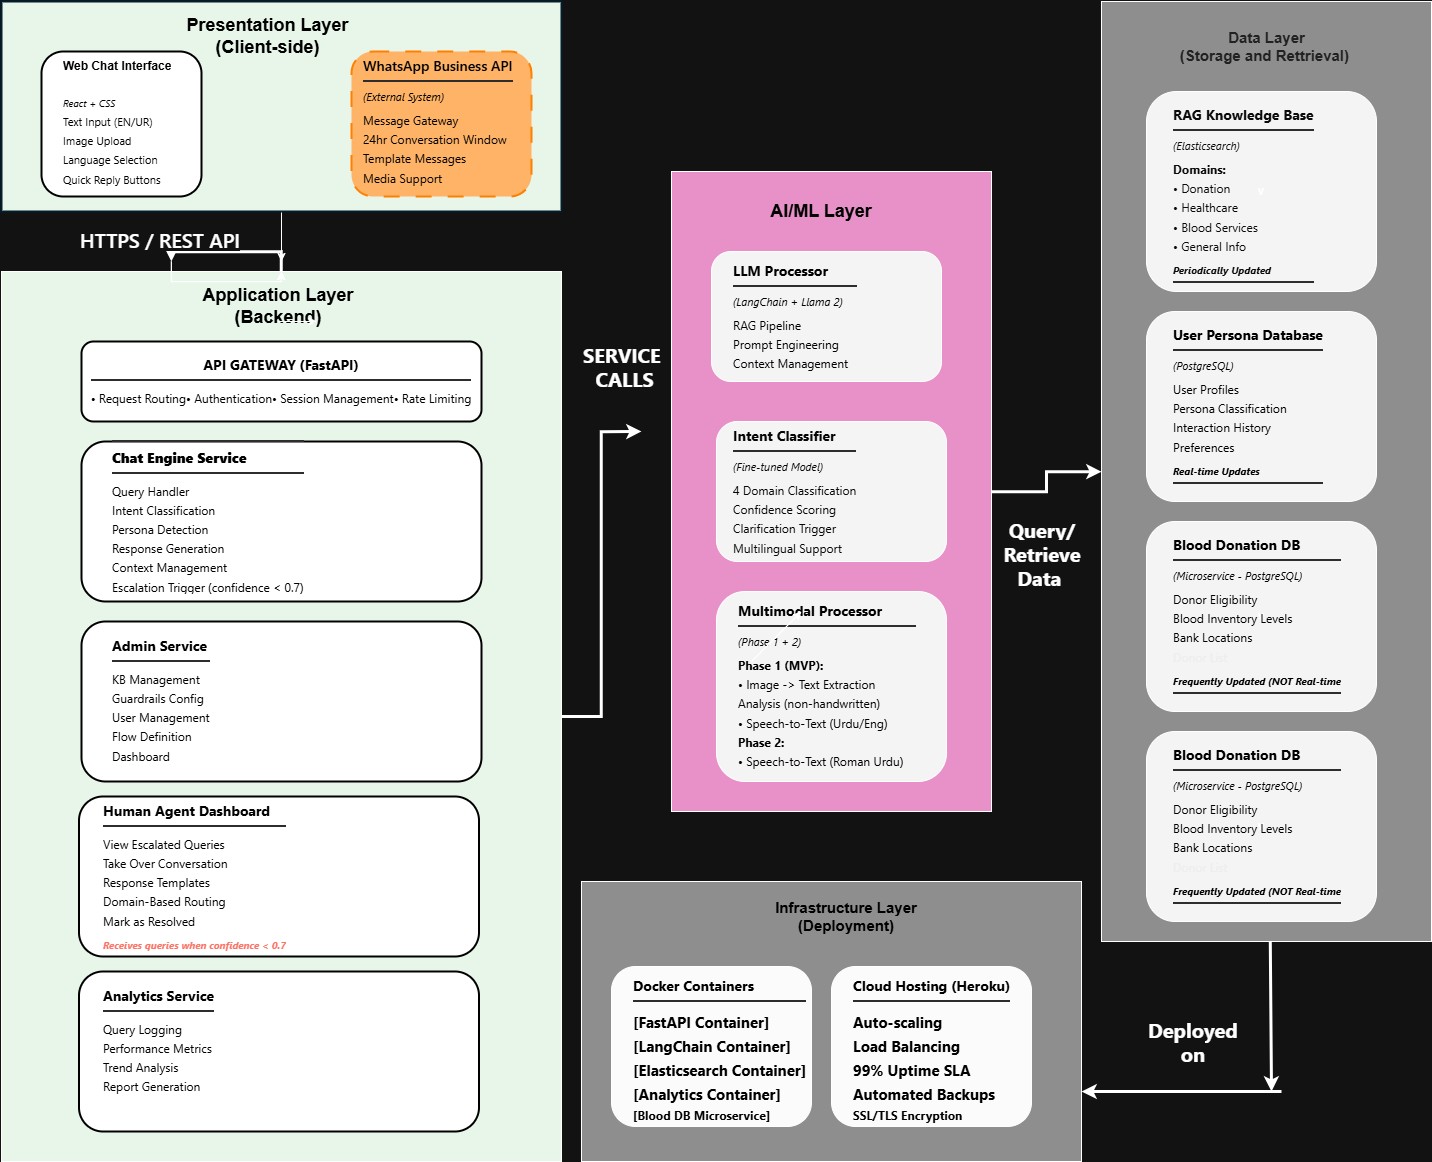
\includegraphics[width=1.1\textwidth]{chapters/high_level_architecture.drawio (1).png}
    \caption{High-level System Architecture}
    \label{fig:sysarchitecture}
\end{figure}
To view the diagram clearly, kindly access the following \href{https://app.diagrams.net/#G19okfbdDRLwywSZxlLuuXVhx5-wa4h22O#%7B%22pageId%22%3A%22drq8IgXnazhB2lmtOcQS%22%7D}{link.}
\\
The proposed system follows a five-layer architecture: Presentation Layer, Application Layer, AI/ML Layer, Data Layer, and Infrastructure Layer. Each layer plays a distinct role in ensuring efficient communication, scalability, and performance.

\subsection{Presentation Layer (Client-Side)}

\textbf{Components:}
\begin{itemize}
    \item \textbf{Web Chat Interface:} Built using React and CSS, enabling the user to interact with the system through a web interface. It supports features like text input (EN/UR), image uploads, language selection, and quick reply buttons.
    \item \textbf{WhatsApp Business API:} Used for external messaging functionalities such as managing conversations within a 24-hour window, sending template messages, and supporting media in chats.
\end{itemize}

\textbf{Role:} This layer is responsible for presenting the interface to the user, collecting user inputs, and initiating requests to the application layer via HTTP/REST APIs.

\subsection{Application Layer (Backend)}

\textbf{Components:}
\begin{itemize}
    \item \textbf{API Gateway:} Manages incoming requests, handles authentication, session management, and rate limiting.
    \item \textbf{Chat Engine Service:} Handles the main logic for query processing, intent classification, persona detection, and response generation. It also includes context management and escalation triggers for low-confidence queries.
    \item \textbf{Admin Service:} Provides tools for managing the knowledge base, user roles, and defining conversation flows.
    \item \textbf{Human Agent Dashboard:} Assists human agents in handling escalated queries, managing conversations, and routing them based on specific domains.
    \item \textbf{Analytics Service:} Logs queries, monitors performance metrics, and generates reports on system usage and trends.
\end{itemize}

\textbf{Role:} This layer is where the core processing happens. It handles requests from the presentation layer, processes them using the chat engine, and provides feedback to the user.

\subsection{AI/ML Layer}

\textbf{Components:}
\begin{itemize}
    \item \textbf{LLM Processor:} Processes the natural language input using large language models (LLMs) such as LangChain and Llama~2. It performs tasks like prompt engineering and context management.
    \item \textbf{Intent Classifier:} Classifies user inputs into predefined domains, scores confidence levels, and triggers escalation when confidence is low.
    \item \textbf{Multimodal Processor:} Handles input types like images or non-handwritten text and processes them into usable information, including support for Urdu and Roman Urdu.
\end{itemize}

\textbf{Role:} The AI/ML layer enhances the system's ability to process and understand user queries, making it capable of handling diverse input types and languages while maintaining context for more accurate responses.

\subsection{Data Layer (Storage and Retrieval)}

\textbf{Components:}
\begin{itemize}
    \item \textbf{RAG Knowledge Base:} Stores structured data related to donation, healthcare, and general services. This database is periodically updated.
    \item \textbf{User Persona Database:} Tracks user profiles, including interaction history, preferences, and persona classification, to provide personalized responses.
    % \item \textbf{Blood Donation Database:} Contains critical data on donor eligibility, blood inventory levels, and bank locations. This database is frequently updated.
\end{itemize}

\textbf{Role:} The data layer ensures that the necessary information is available for the application layer to process and retrieve during interactions. It stores both real-time and frequently updated data for accurate responses.

\subsection{Infrastructure Layer (Deployment)}

\textbf{Components:}
\begin{itemize}
    \item \textbf{Docker Containers:} Each component, including the FastAPI service, LangChain, Elasticsearch, and analytics, is containerized to ensure consistent and scalable deployment.
    \item \textbf{Cloud Hosting (Heroku):} The system is hosted on Heroku with auto-scaling, load balancing, and high availability (99\% uptime SLA). SSL/TLS encryption ensures secure communication.
\end{itemize}

\textbf{Role:} The infrastructure layer ensures that the system is deployed efficiently, scalable, and resilient. It handles the deployment of services and ensures they are readily available to process requests.

\subsection{Relationships Between Layers}

\begin{itemize}
    \item User interaction starts at the \textbf{Presentation Layer}, where the user inputs queries.
    \item Requests are routed via HTTPS/REST APIs to the \textbf{Application Layer} for processing.
    \item The \textbf{Chat Engine Service} in the Application Layer utilizes the \textbf{AI/ML Layer} to classify intents and process natural language queries.
    \item \textbf{Data Retrieval} from the Data Layer occurs through queries made by application services, which fetch relevant data from the knowledge base and databases.
    \item The system is deployed on the \textbf{Infrastructure Layer}, ensuring scalability and security.
\end{itemize}

\subsection{Flow of Interaction}

\begin{enumerate}
    \item \textbf{User Interaction} $\rightarrow$ Presentation Layer $\rightarrow$ API Gateway
    \item \textbf{Request Routing} $\rightarrow$ Chat Engine Service $\rightarrow$ AI/ML Layer (Intent Classification \& Response Generation)
    \item \textbf{Data Retrieval} $\rightarrow$ Data Layer (RAG Knowledge Base, User Persona)
    \item \textbf{Response Sent} $\rightarrow$ Presentation Layer $\rightarrow$ User (via WhatsApp or Web Chat)
\end{enumerate}

This architecture ensures that each layer is responsible for a specific aspect of the system, from front-end interaction to backend processing, AI-based intent classification, and data management, all underpinned by scalable and secure infrastructure.


\section{External Interfaces}
\subsection{User Interfaces - Wireframes}
% This section includes our mockup screens and briefly explains them.
\begin{figure}[H]
    \centering
    \includegraphics[width=1\textwidth]{chapters/whatsapp_ui.png}
    % 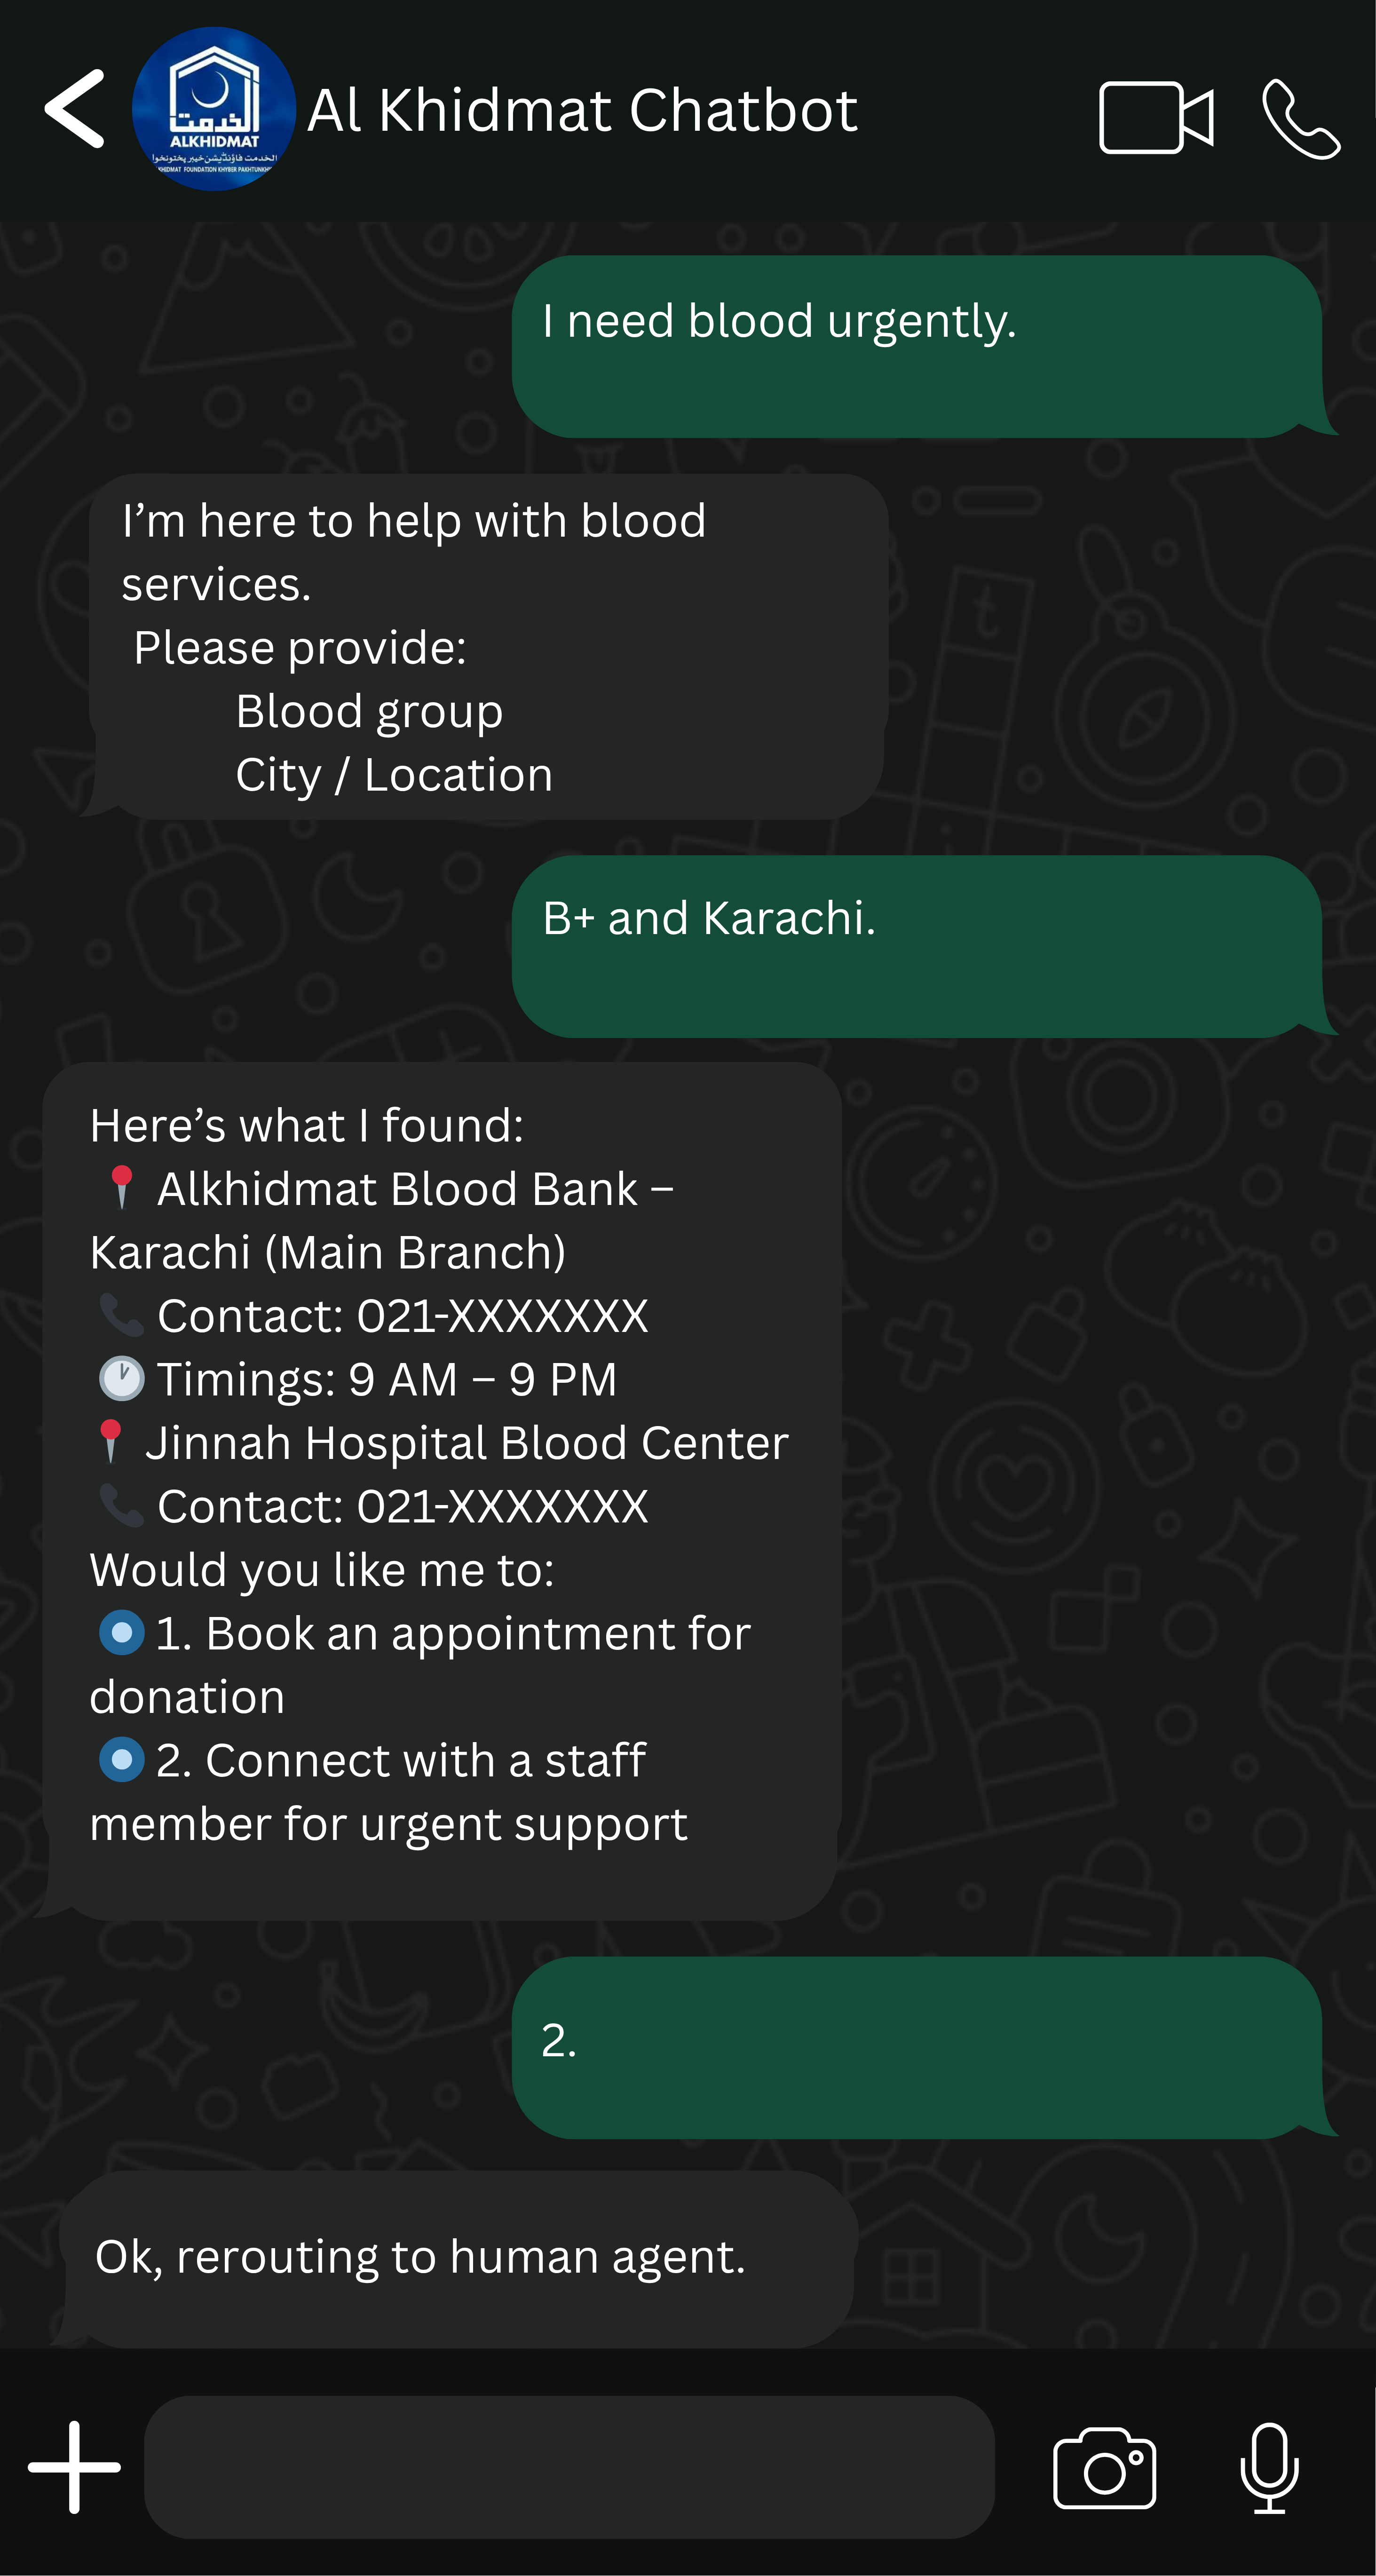
\includegraphics[width=0.335\textwidth]{chapters/chat2.png}
    \caption{User Interface using Whatsapp}
    \label{fig:UIuser}
\end{figure}

The two wireframes show how users might interact with the AI chatbot. Here, two use-cases are shown; monetary donors can select between Zakat, Sadaqah, or General Donations using quick buttons, receive verified payment options (Easypaisa, JazzCash, Visa/MasterCard), and obtain secure links with automated receipts, while complex or high-value cases are routed to human donation officers. Similarly, users seeking blood support can provide their blood group and city to instantly retrieve nearby Alkhidmat blood bank details and contact numbers; for urgent or unclear cases, the chatbot escalates the conversation to a live human agent within the same WhatsApp thread as we see in below wireframes. Both flows ensure verified information, user-friendly navigation, and human oversight for transparency and reliability.
\newpage
\begin{figure}[H]
    \centering
    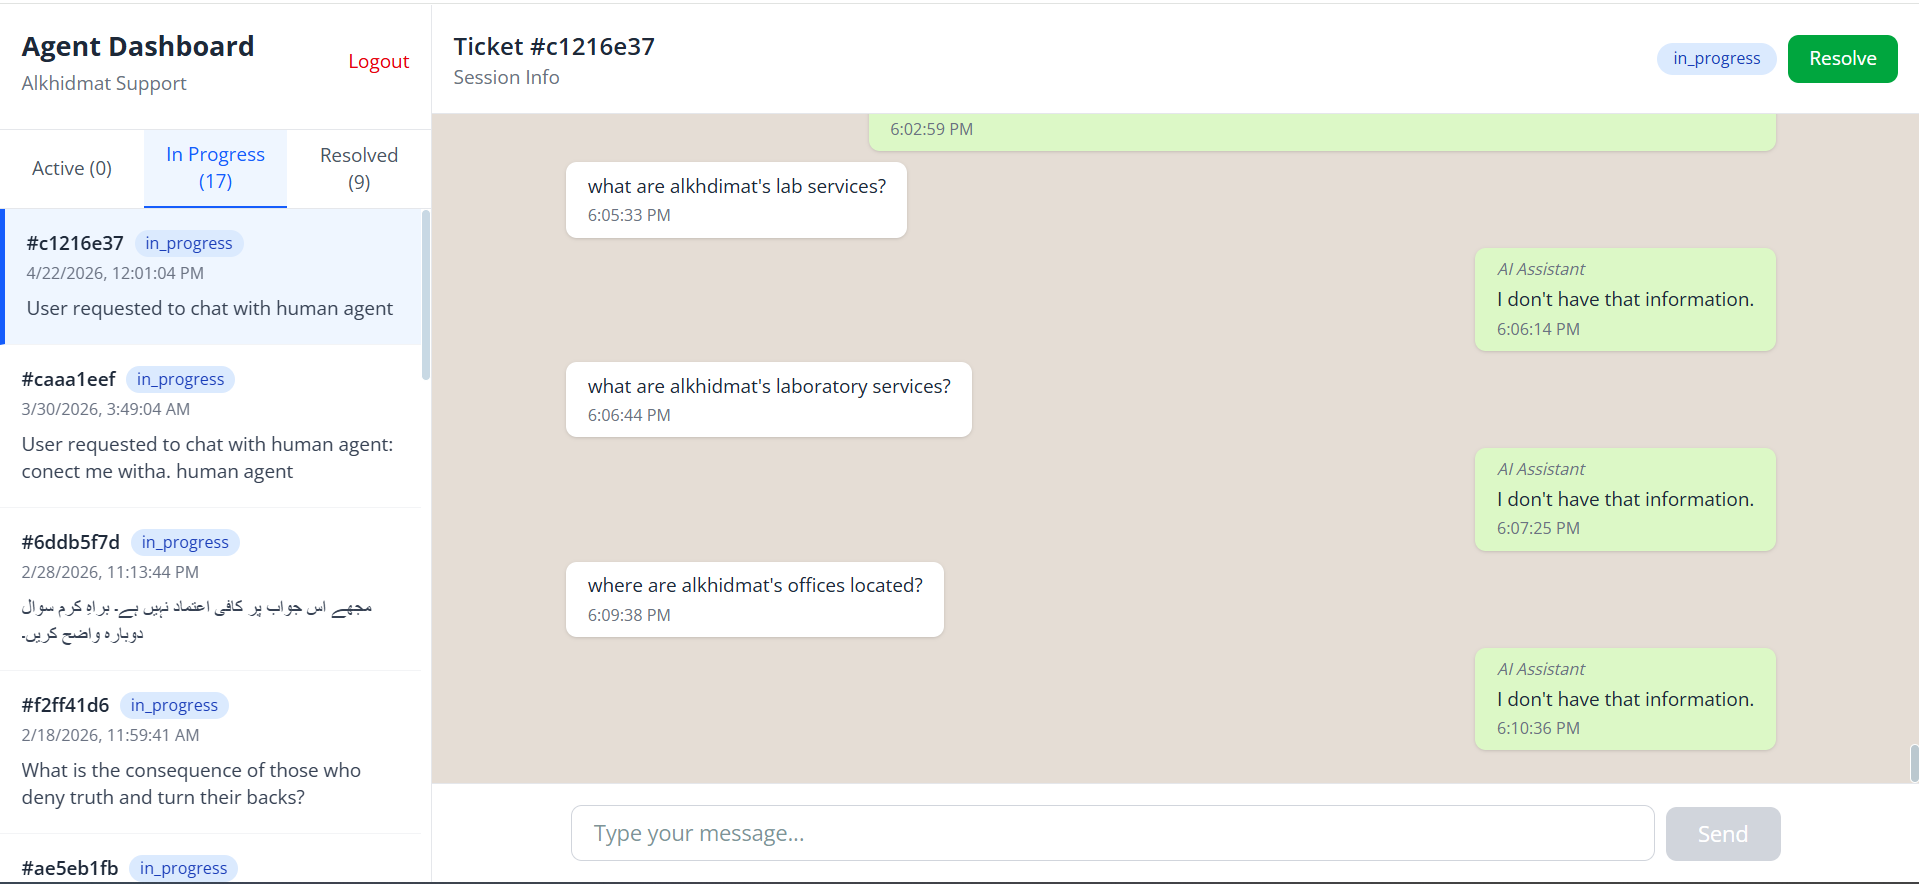
\includegraphics[width=1\textwidth]{chapters/Staff dashboard.png}
    \caption{Staff Dashboard}
    \label{fig:staffdashboard}
\end{figure}
If the AI bot is unable to confidently resolve any query, it will be escalated to Al-Khidmat's staff. The following is the dashboard where they will receive the queries.\\
The following example shows that the AI bit resolved a query with 8\% confidence, so it has been escalated to Fatima Ahmed, a human agent. She sees that there is a new ticket. She reviews the context where the user asked sensitive information and would personally guide her - all while updating the knowledge base for future training.
\\
The dashboard includes:
\begin{itemize}\setlength{\itemsep}{0pt}
    \item Left Panel: Live ticket queue with 4 realistic escalation scenarios (medical emergency, zakat calculation, scholarship, etc)
    \item Center Panel: Bilingual conversation thread showing bot-to-human handoff, where the agent has an option to transfer the query to another agent and resolve it once completed.
    \item Right Panel: User profile, escalation metadata, and knowledge base update form
\end{itemize}
\begin{figure}[H]
    \centering
    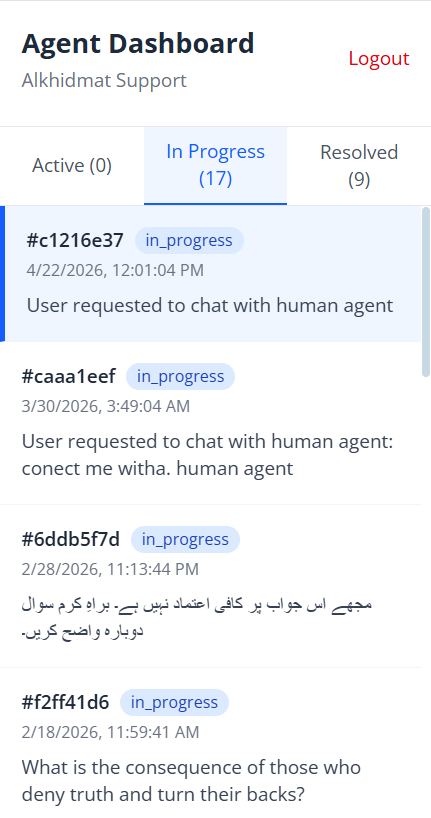
\includegraphics[width=0.5\textwidth]{chapters/ticket.png}
    \caption{Further Contents in Ticket Content Panel}
    \label{fig:ticketcontent1}
\end{figure}
% \begin{figure}[H]
%     \centering
%     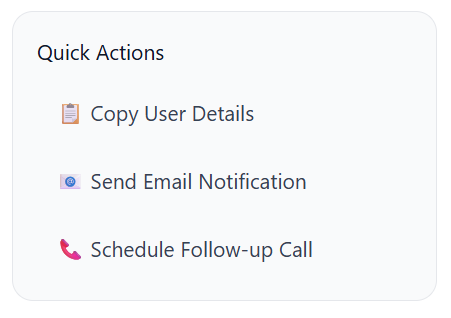
\includegraphics[width=0.5\textwidth]{chapters/Ticket Content 2.png}
%     \caption{Further Contents in Ticket Content Panel}
%     \label{fig:ticketcontent2}
% \end{figure}

\begin{figure}[H]
    \centering
    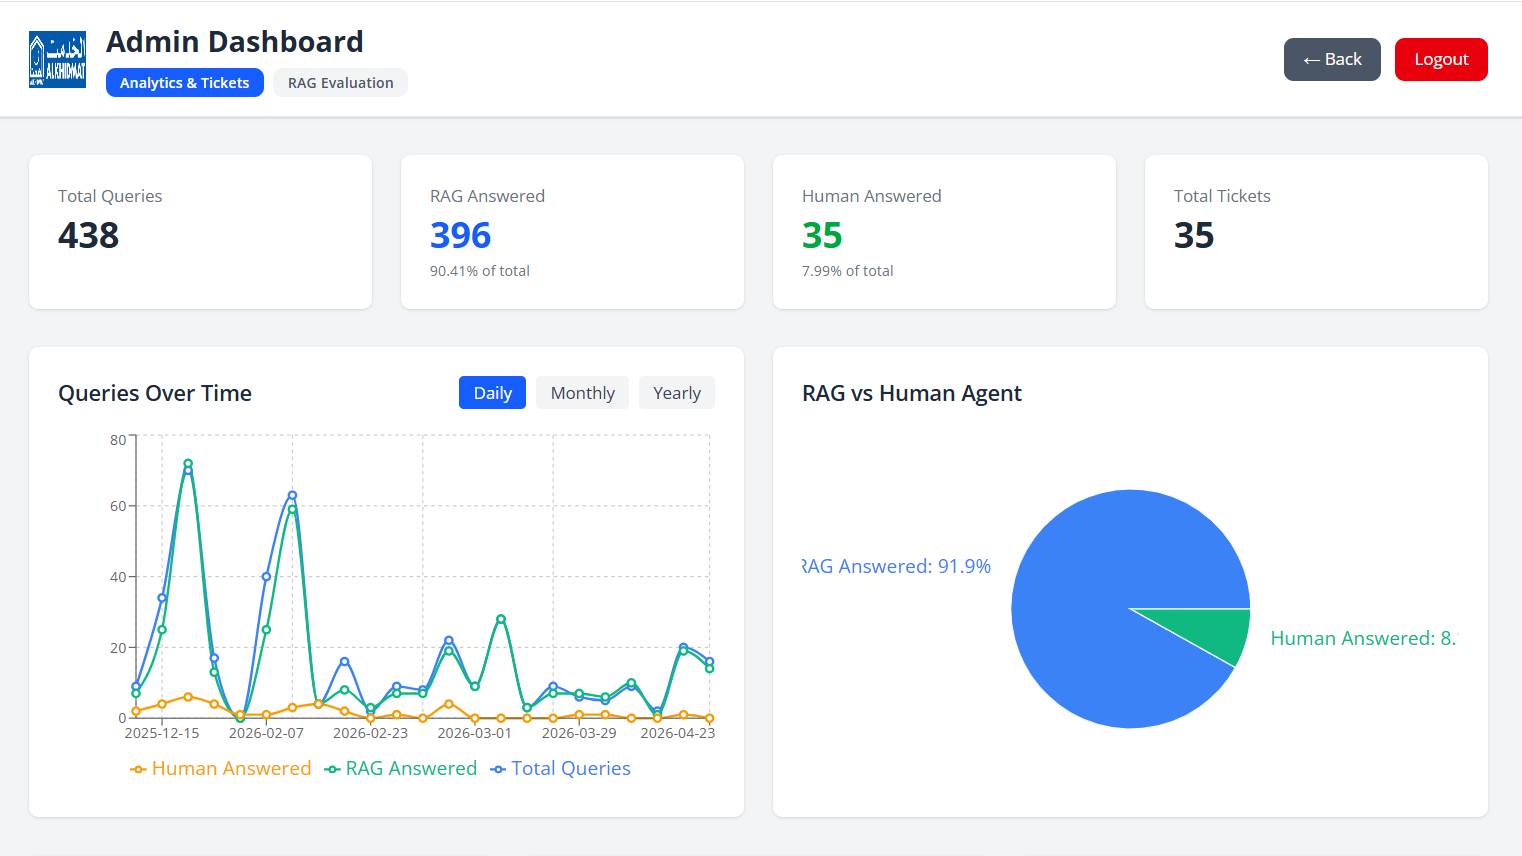
\includegraphics[width=0.9\textwidth]{chapters/dashboard.png}
    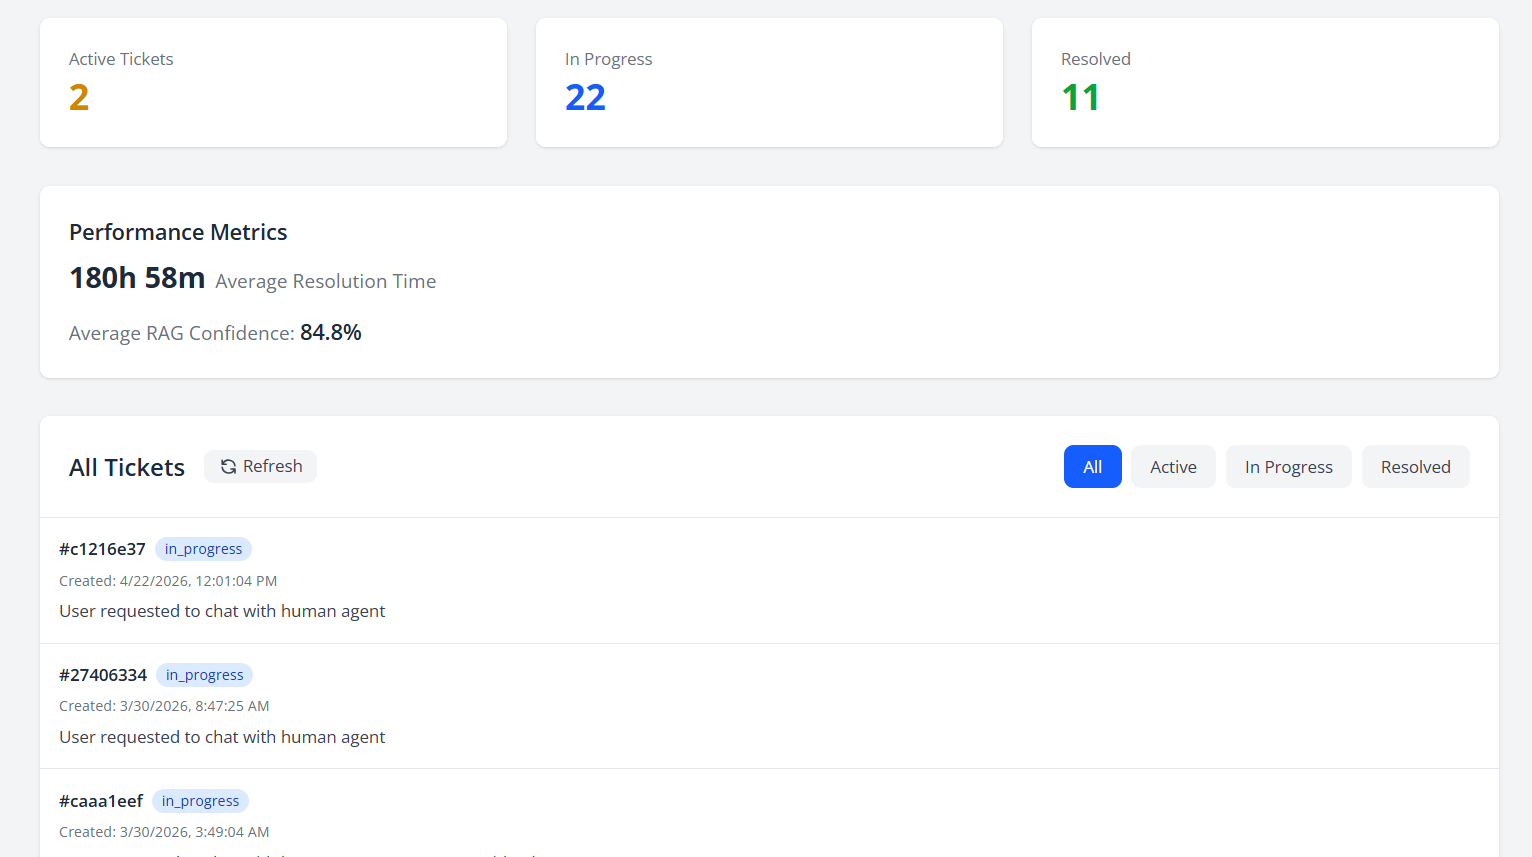
\includegraphics[width=0.9\textwidth]{chapters/dashboard_1.png}
    \caption{Admin's Dashboard - Analytics Monitor}
    \label{fig:analytics}
\end{figure}

The Analytics Dashboard features real-time tracking of chatbot performance and user activity, including domain-wise query distribution, daily and hourly interaction trends, and key usage metrics like total queries, average session time, and peak hours. It provides detailed insights into escalation rates, comparing AI-handled and human-assisted queries across domains to assess accuracy and efficiency. Additional features include a date selector for reviewing past analytics, visual charts for quick interpretation, and an intuitive, admin-friendly interface aligned with Alkhidmat Foundation’s branding for easy monitoring and performance optimization.

\begin{figure}[H]
    \centering
    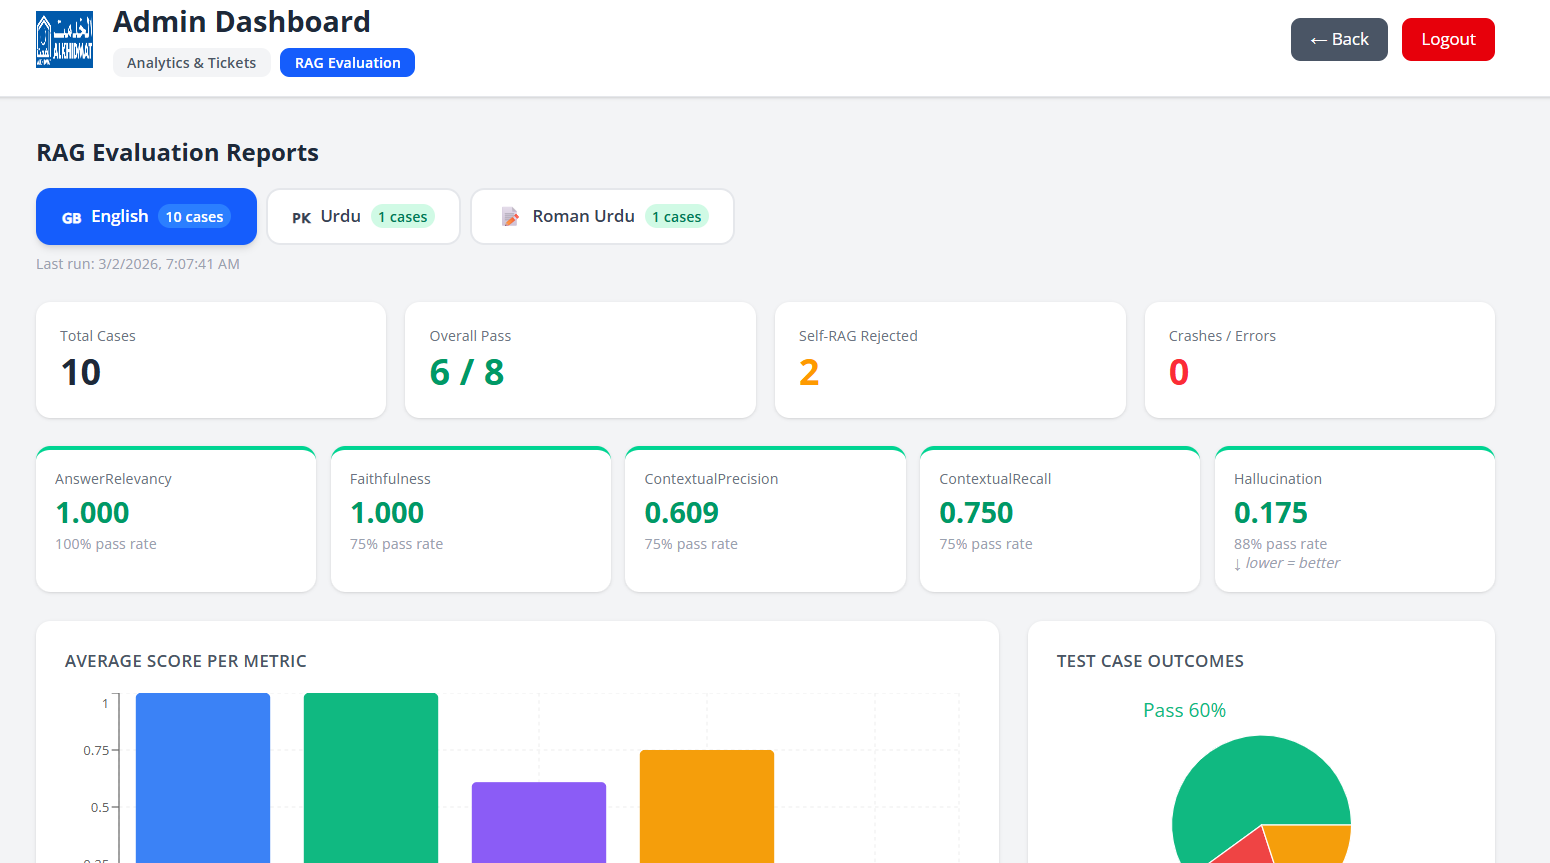
\includegraphics[width=0.9\textwidth]{chapters/RAG_eval.png}
    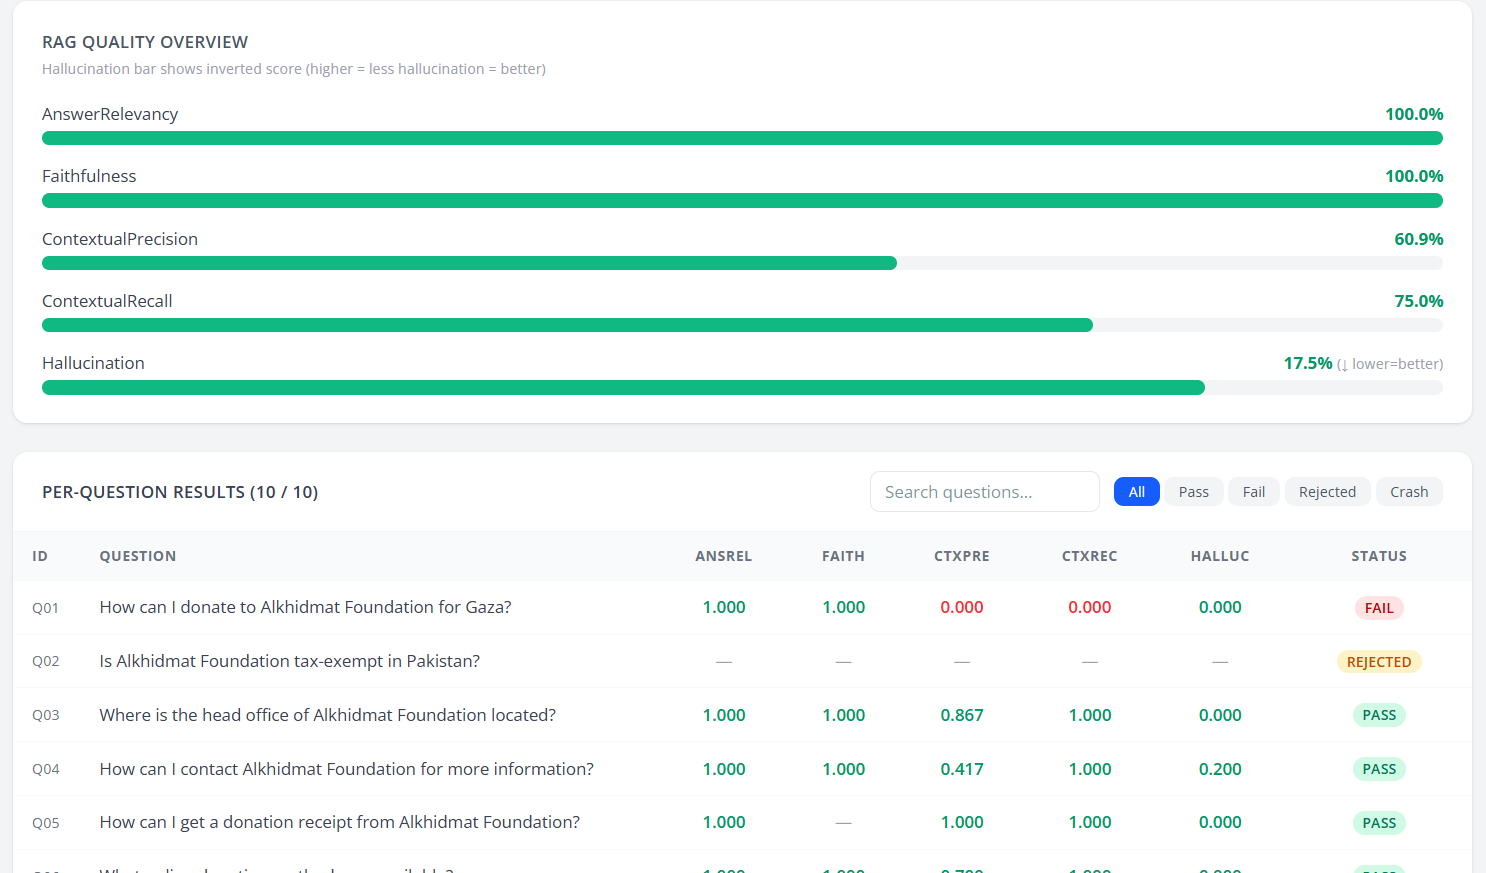
\includegraphics[width=0.9\textwidth]{chapters/RAG_eval_1.png}  
    \caption{Admin's Dashboard - RAG Evaluation}
    \label{fig:analytics_1}
\end{figure}
% \section{External Interfaces}

% We expect every project to have at least of the following subsections. This section must be aligned with your project deliverables. Please consult with your project supervisor regarding which of the following section(s) you should include in your report

% \subsection{Application Program Interface (API)}
% This section describes the library or API interface to our system.

% \subsection{Hardware/Communication Interfaces}
% This section describes our project's specific hardware/network interfaces.

% \section{Datasets}
% This section describes the specific dataset(s) used to build our system. An appropriate snapshot of the dataset(s) is also included. Futher details, when needed, are presented in the appendix.



\chapter{Software Design Specification (SDS)}
\label{chap:sds}
\section{Software Design}

\subsection{High-Level Architecture (textual)}
Five-layer architecture (as in SRS) — component view and interaction flow.

\textbf{Interaction flow (short):}
\begin{quote}
Client $\rightarrow$ API Gateway $\rightarrow$ Chat Engine $\rightarrow$ (Intent Classifier $\rightarrow$ RAG Retrieval + LLM) $\rightarrow$ Response $\rightarrow$ Presentation.
\end{quote}

Escalation path sends conversation + context to Human Agent Dashboard; Human updates KB via Admin Service.

\subsection{Component/Service Summary}
Below are the top-level services (each top-level class may map to a microservice).

\begin{itemize}
  \item \textbf{APIGateway} — Authentication, rate-limiting, routing, request validation.
  \item \textbf{ChatEngine} — Orchestrates conversational processing, session management, calls ML services.
  \item \textbf{AdminService} — KB CRUD, guardrails, role management.
  \item \textbf{HumanDashboard} (HumanAgent) — Agent UI/API for escalations and KB updates.
  \item \textbf{AnalyticsService} — Logs metrics, calculates KPIs, anomaly alerts.
  \item \textbf{IntentClassifier} — Predicts intent/domain with confidence scores.
  \item \textbf{MultimodalProcessor} — Image OCR, document classification, entity extraction.
  \item \textbf{RAGEngine} — Vector search + LLM prompt generation and answer synthesis.
  \item \textbf{DataStore} — Relational DB (Postgres), vector store (FAISS/Milvus/Elastic vectors), cache (Redis).
\end{itemize}

\subsection{UML}
Below is a UML diagram describing the UML class/service relationships.
\begin{figure}[h!]
    \centering
    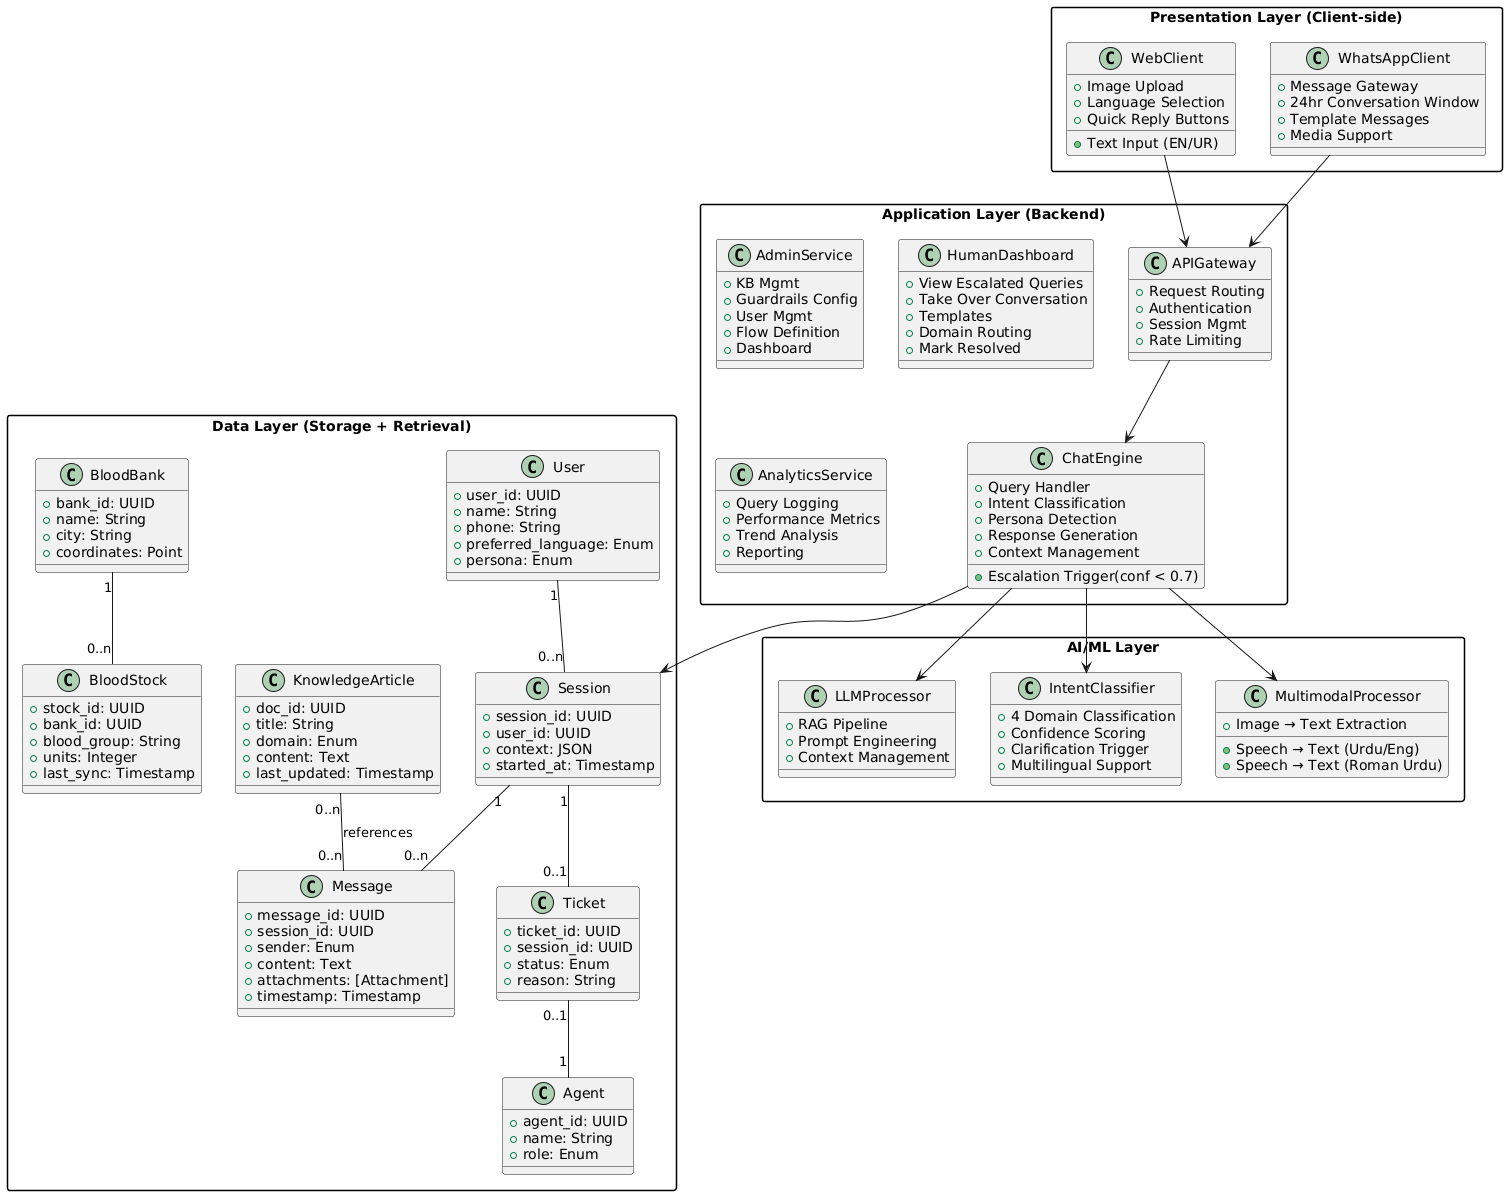
\includegraphics[width=0.95\linewidth]{chapters/UML.png}
    \caption{UML Diagram}
    \label{fig:placeholder}
\end{figure}
\subsection{Classes - Descriptions}
Below are concise descriptions, attributes and methods for the main classes/services.

\subsubsection{APIGateway}
\textbf{Purpose:} Authentication, rate-limiting, routing to backend services, request validation.  
\textbf{Attributes:} tokenStore (JWT secret), rateLimitConfig.  
\textbf{Methods:} \texttt{authenticate(req)}, \texttt{authorize(req)}, \texttt{route(req)}, \texttt{rateLimit(req)}.  
\textbf{Relationships:} front door for WebClient \& WhatsAppClient $\rightarrow$ ChatEngine, AdminService.

\subsubsection{ChatEngine}
\textbf{Purpose:} Orchestrates conversational processing: receives messages, manages sessions, calls intent classifier, multimodal processor, RAG engine, returns responses and handles escalation.  
\textbf{Attributes:} sessionStore (Redis), kbClient, classifierClient, ragClient, escalationPolicy.  
\textbf{Methods:}
\begin{itemize}
  \item \texttt{processIncoming(message: Message)}
  \item \texttt{classifyIntent(text) $\rightarrow$ IntentResult}
  \item \texttt{handleMultimodal(attachments) $\rightarrow$ structured artifacts}
  \item \texttt{generateResponse(context) $\rightarrow$ final message}
  \item \texttt{escalate(session, reason) $\rightarrow$ creates Ticket}
\end{itemize}
\textbf{Relationships:} calls IntentClassifier, MultimodalProcessor, RAGEngine, DataStore.

\subsubsection{AdminService}
\textbf{Purpose:} CRUD for knowledge base, guardrails, role management.  
\textbf{Attributes:} KBRepository, userManager.  
\textbf{Methods:} \texttt{createArticle()}, \texttt{updateArticle()}, \texttt{publishKBVersion()}, \texttt{setGuardrails()}.

\subsubsection{HumanDashboard}
\textbf{Purpose:} Staff-facing UI/API for taking over escalated tickets, replying to users, updating KB.  
\textbf{Attributes:} ticketQueue, websocketConnections.  
\textbf{Methods:} \texttt{claimTicket(ticketId)}, \texttt{postReply(ticketId, message)}, \texttt{updateKBFromInteraction(...)}.

\subsubsection{AnalyticsService}
\textbf{Purpose:} Log metrics, build KPIs.  
\textbf{Attributes:} metricsStore, logDB.  
\textbf{Methods:} \texttt{logQuery(...)} , \texttt{getKPI(start,end)}, \texttt{alertAnomalies()}.

\subsubsection{AI/ML Services}
\textbf{IntentClassifier:} model (transformer or embed+classifier), \texttt{predict(text)} $\rightarrow$ \{intent, domain, confidence, top\_k\}.  
\textbf{MultimodalProcessor:} visionModel, ocrEngine, imagePreproc, \texttt{processImage(img)}.  
\textbf{RAGEngine:} vectorStore, index, llmClient, promptTemplates, \texttt{retrieve(query,k)}, \texttt{buildPrompt(context, docs)}, \texttt{generateAnswer(prompt)}.

\subsubsection{Data-layer domain models}
\textbf{User, Session, Message, Ticket, KnowledgeArticle, Agent, BloodBank, BloodStock, AuditLog} — attributes and typical service-level methods (getProfile, loadContext, serialize, assign, resolve, searchIndex).

\section{Data Design}

\subsection{Entities, PK/FK and Cardinalities (summary)}
\begin{itemize}
  \item \textbf{User (1) -- (0..n) Session} : A user can have many sessions.
  \item \textbf{Session (1) -- (0..n) Message} : A session has many messages.
  \item \textbf{Session (1) -- (0..1) Ticket} : A session may create a ticket.
  \item \textbf{Ticket (0..n) -- (0..1) Agent} : Tickets can be assigned to an agent.
  \item \textbf{KnowledgeArticle (0..n) -- (0..n) Message} : Many-to-many via junction table message\_article\_refs.
  \item \textbf{BloodBank (1) -- (0..n) BloodStock} : Each bank has multiple stock entries.
\end{itemize}

\subsection{Relational Schema (core tables) — SQL DDL}
Below are simplified Postgres table definitions for core tables. In production add indexes, constraints, partitioning, and tuning.

\begin{lstlisting}[language=SQL]
-- Users
CREATE TABLE users (
  user_id UUID PRIMARY KEY,
  name TEXT,
  phone TEXT,
  email TEXT,
  preferred_language TEXT,
  created_at TIMESTAMP WITH TIME ZONE DEFAULT now()
);

-- Sessions
CREATE TABLE sessions (
  session_id UUID PRIMARY KEY,
  user_id UUID REFERENCES users(user_id),
  started_at TIMESTAMP WITH TIME ZONE DEFAULT now(),
  last_active_at TIMESTAMP WITH TIME ZONE DEFAULT now(),
  context JSONB
);

-- Messages
CREATE TABLE messages (
  message_id UUID PRIMARY KEY,
  session_id UUID REFERENCES sessions(session_id) ON DELETE CASCADE,
  sender TEXT,
  content TEXT,
  attachments JSONB,
  timestamp TIMESTAMP WITH TIME ZONE DEFAULT now(),
  intent_label TEXT,
  confidence NUMERIC
);

-- Tickets
CREATE TABLE tickets (
  ticket_id UUID PRIMARY KEY,
  session_id UUID REFERENCES sessions(session_id),
  status TEXT,
  assigned_to UUID, -- references agents.agent_id (create agents table below)
  priority TEXT,
  reason TEXT,
  created_at TIMESTAMP WITH TIME ZONE DEFAULT now(),
  resolved_at TIMESTAMP WITH TIME ZONE
);

-- Knowledge articles
CREATE TABLE knowledge_articles (
  doc_id UUID PRIMARY KEY,
  title TEXT,
  content TEXT,
  domain TEXT,
  tags TEXT[],
  source_url TEXT,
  last_updated TIMESTAMP WITH TIME ZONE,
  version INTEGER
);

-- Message <-> Article references (junction)
CREATE TABLE message_article_refs (
  id UUID PRIMARY KEY,
  message_id UUID REFERENCES messages(message_id),
  doc_id UUID REFERENCES knowledge_articles(doc_id)
);

-- Agents
CREATE TABLE agents (
  agent_id UUID PRIMARY KEY,
  name TEXT,
  roles TEXT[],
  email TEXT,
  active BOOLEAN DEFAULT true
);

-- Blood bank and stock
CREATE TABLE blood_banks (
  bank_id UUID PRIMARY KEY,
  name TEXT,
  address TEXT,
  city TEXT,
  coordinates POINT,
  contact TEXT
);

CREATE TABLE blood_stock (
  stock_id UUID PRIMARY KEY,
  bank_id UUID REFERENCES blood_banks(bank_id) ON DELETE CASCADE,
  blood_group TEXT,
  units_available INTEGER,
  last_updated TIMESTAMP WITH TIME ZONE
);
-- Unique constraint to prevent duplicate (bank_id, blood_group)
ALTER TABLE blood_stock
  ADD CONSTRAINT uniq_bank_group UNIQUE (bank_id, blood_group);

-- Audit logs
CREATE TABLE audit_logs (
  log_id UUID PRIMARY KEY,
  actor_id UUID,
  action TEXT,
  details JSONB,
  timestamp TIMESTAMP WITH TIME ZONE DEFAULT now()
);
\end{lstlisting}

\subsection{Indexes and Search}
\begin{itemize}
  \item Full-text search: add \texttt{tsvector} columns and GIN indexes on \texttt{knowledge\_articles(content, title)}.
  \item Vector embeddings: store in a vector store (FAISS/Milvus/Elastic vector index) keyed by \texttt{doc\_id}. Keep metadata in a \texttt{kb\_index} table linking \texttt{doc\_id} $\rightarrow$ vector\_id.
  \item Cache hot items in Redis. Use LRU eviction for cache.
\end{itemize}

\subsection{Normalization \& Cardinalities Rationale}
Schema is in 3NF:
\begin{itemize}
  \item KB articles separated from message-level references to avoid duplication.
  \item Sessions store transient conversation context; messages are transactional and cascade on session deletion.
  \item Blood\_stock uses unique constraint on (bank\_id, blood\_group) to avoid duplication and simplify updates.
  \item message\_article\_refs preserves KB provenance for each response.
\end{itemize}

\section{Technical Details — Algorithms \& Implementation Notes}

For each pipeline I list purpose, inputs/outputs, steps (pseudocode), placement, complexity, failure modes and mitigations.

\subsection{Incoming Message Pipeline (Orchestration)}
\textbf{Purpose:} End-to-end handling of a user message: preproc $\rightarrow$ intent $\rightarrow$ retrieval/generation $\rightarrow$ response or escalate.  
\textbf{Placement:} ChatEngine service.

\textbf{Input:} Message (text + optional attachments + user\_id + session\_id).  
\textbf{Output:} Response (text, attachments, metadata), or created Ticket.

\textbf{Pseudocode:}
\begin{lstlisting}
function processIncoming(msg):
  session = SessionStore.get(msg.session_id)
  preproc_text = normalize_text(msg.content, user_lang=session.pref_lang)
  if msg.attachments present:
    image_info = MultimodalProcessor.process(msg.attachments)
    enrich context with image_info

  intent_result = IntentClassifier.predict(preproc_text)
  if intent_result.confidence < CONFIDENCE_THRESHOLD (0.7):
    create_ticket(session, reason='low_confidence', msg)
    return respond_with_escalation_notice()
  
  docs = RAGEngine.retrieve(preproc_text, k=5)
  prompt = RAGEngine.buildPrompt(session.context, preproc_text, docs)
  answer, sources = RAGEngine.generateAnswer(prompt)
  
  persona = PersonaService.get(session.user_id)
  answer = PersonaService.format(answer, persona)
  
  Analytics.log(query, intent_result, latency)
  MessageStore.saveBotResponse(session, answer, sources)
  return answer
\end{lstlisting}

\textbf{Complexity:} Vector retrieval typically sub-linear; LLM generation dominates latency and cost.  
\textbf{Failure modes:} LLM hallucination, outdated KB — mitigate by returning explicit sources, confidence, and allowing human escalation.

\subsection{Intent Classification}
\textbf{Purpose:} Route queries by domain and decide escalation.

\textbf{Options:}
\begin{description}
  \item[Option A (recommended):] Transformer fine-tuned classifier (small BERT / DistilBERT) for multilingual support.
  \item[Option B:] Embedding + k-NN for low-resource scenarios.
\end{description}

\textbf{Pseudocode:}
\begin{lstlisting}
predict(text):
  tokens = tokenizer(text)
  probs = model.forward(tokens)  -- softmax per class
  label = argmax(probs)
  confidence = probs[label]
  return {label, confidence}
\end{lstlisting}

\textbf{Notes:} Confidence threshold = 0.7. Return top\_k candidate intents for clarification loops. Use data augmentation for Roman Urdu.

\subsection{RAG Retrieval \& Generation Pipeline}
\textbf{Purpose:} Factually-grounded LLM responses using KB documents.

\textbf{Steps:}
\begin{enumerate}
  \item Preprocess query (language, entity extraction).
  \item Embed query; vector search top-k (k=5--10).
  \item Rerank by metadata (city, blood group, last\_updated).
  \item Build structured prompt with system instruction + context + doc excerpts + provenance.
  \item Call LLM to generate answer.
  \item Post-process: sanitize, attach citations, compute heuristic confidence.
\end{enumerate}

\textbf{Pseudocode:}
\begin{lstlisting}
docs = vector_search(query, k)
docs = rerank_by_metadata(docs, query_entities)
prompt = build_prompt(context, query, docs)
answer = llm.generate(prompt)
sources = extract_sources(answer, docs)
\end{lstlisting}

\textbf{Notes:} Use chunking for long docs, prioritize recently-updated docs for time-sensitive queries (e.g., blood availability). Add guardrails to prevent PII exposure.

\subsection{Multimodal Processing (Image Handling)}
\textbf{Purpose:} Extract text and structured info from images (receipts, prescriptions, confirmations).

\textbf{Steps:}
\begin{itemize}
  \item Preprocess image (resize, denoise).
  \item Doc-type classification: CNN predicts receipt/prescription/ID/photo.
  \item Run OCR (Tesseract or cloud).
  \item Entity extraction: NER or regex on OCR text (txn\_id, date, hospital).
  \item Return structured JSON to ChatEngine.
\end{itemize}

\textbf{Limitations:} Handwritten recognition out-of-scope for MVP; low-quality images return low-confidence and prompt user to reupload.

\subsection{Persona Classification \& Response Personalization}
\textbf{Purpose:} Tailor tone, verbosity, and suggestions based on the persona (donor type, patient type).

\textbf{Technique:} Rule-based + light ML classifier using session history, language, frequency. Persona stored in Redis or persona\_profile table.

\subsection{Escalation Logic (Human Handoff)}
\textbf{Purpose:} Move low-confidence or sensitive queries to human agents preserving context.

\textbf{Rules:}
\begin{itemize}
  \item intent.confidence < 0.7 $\rightarrow$ escalate.
  \item Sensitive patterns (refund, complaint, PII requests) $\rightarrow$ escalate.
  \item user explicitly requests human $\rightarrow$ escalate.
\end{itemize}

\textbf{Steps:}
\begin{enumerate}
  \item Create ticket with snapshot context.
  \item Notify agent queue (domain-based).
  \item Lock session for human takeover.
  \item Agent replies via Dashboard; ChatEngine relays reply.
  \item Agent may update KB \& resolve ticket.
\end{enumerate}

\subsection{Session Management \& Context Windowing}
\textbf{Purpose:} Maintain multi-turn context while staying below LLM prompt limits.

\textbf{Technique:} Keep full short context in Redis; for long histories summarize early messages into compact structured fields (last\_intent, open\_issues, recent\_entities) and include recent N messages directly.

\subsection{Caching \& Performance}
\textbf{Layers:}
\begin{itemize}
  \item Redis: sessions, persona, short-term query cache.
  \item Persistent cache / warm vector cache: frequently-seen RAG results (TTL e.g., 1h).
\end{itemize}

\textbf{Scaling:} Containerize services horizontally. Vector store and Elasticsearch scaled/sharded as needed.

\subsection{Monitoring, Logging, Analytics}
\textbf{Metrics:} QPS, avg latency, LLM call latency, intent accuracy, escalation rate, KB hit rate, user satisfaction.  
\textbf{Tools:} Prometheus (metrics), Grafana (dashboards), ELK (logs).  
\textbf{Alerts:} High escalation rate, low accuracy, traffic spikes.

\subsection{Data Integrity, Backup \& Compliance}
\begin{itemize}
  \item Weekly snapshots for KB \& relational DB, daily incremental backups for messages/tickets.
  \item Off-site encrypted backups.
  \item Pseudonymize or avoid persisting PII unless explicit consent.
  \item RBAC for Admin/Agent, audit logs required for agent actions.
  \item Follow local data protection rules.
\end{itemize}

\subsection{Security Design}
\begin{itemize}
  \item TLS everywhere.
  \item JWT for session tokens; secrets in a vault.
  \item Input sanitization for prompts; escape user-supplied data.
  \item Rate-limiting; WhatsApp 24-hour window compliance (templates/outbound).
  \item LLM guardrails to block medical diagnoses and PII disclosure.
\end{itemize}

\section{Example Sequence: ``Find nearest blood bank with O+ in Karachi''}
Example interaction flow:
\begin{enumerate}
  \item User: ``I need O+ blood in Karachi now'' (WhatsApp).
  \item APIGateway authenticates request.
  \item ChatEngine retrieves/creates session.
  \item IntentClassifier $\rightarrow$ BloodService (confidence 0.95).
  \item Entities: blood\_group=O+, city=Karachi.
  \item RAGEngine queries BloodStock microservice (filter: city, blood\_group) $\rightarrow$ nearby\_banks[] with availability.
  \item RAGEngine builds reply with nearest banks, contacts, estimated distances, and a quick-action button.
  \item Message sent to user; analytics logged. If stock below threshold, system triggers donor network alert.
\end{enumerate}

\section{Additional Implementation Notes \& Trade-offs}
\begin{itemize}
  \item \textbf{LLM choice:} Local LLaMA2 (privacy, cost) vs hosted OpenAI (language capability). For Urdu/Roman Urdu, RAG may compensate for smaller LLMs.
  \item \textbf{Vector store:} Elastic vector index or FAISS/Milvus; real-time stock requires streaming updates to metadata or direct DB queries.
  \item \textbf{Multilingual support:} Roman Urdu normalization tables, data augmentation.
  \item \textbf{Latency vs accuracy:} Use caching, smaller prompts to lower latency; accept higher latency for complex answers.
  \item \textbf{Human-in-loop:} Agent UX to push KB updates from interactions to keep RAG fresh.
\end{itemize}

\section{Deliverables Usable in Implementation}
\begin{itemize}
  \item PlantUML file (above) — drop-in to generate UML diagram.
  \item SQL DDL (above) — base schema for Postgres.
  \item Pseudocode for pipelines — can be translated into FastAPI + background workers.
  \item Metrics list — ready for Prometheus instrumentation.
\end{itemize}

\section{Risks and Mitigations}
\begin{itemize}
  \item \textbf{Outdated KB:} show last\_updated timestamps; explicit sources; escalate to humans.
  \item \textbf{Roman Urdu variability:} curated normalization and data augmentation.
  \item \textbf{WhatsApp 24-hour window:} use pre-approved templates; agents respect window.
  \item \textbf{Privacy risks:} minimal PII storage, anonymize logs, strong access controls and encryption.
\end{itemize}

\section{Appendices}

\subsection{Appendix A: Process Pseudocode (processIncoming \& escalate)}
\begin{lstlisting}
-- processIncoming (high-level)
function processIncoming(msg):
  session = SessionStore.get(msg.session_id)
  preproc_text = normalize_text(msg.content, user_lang=session.pref_lang)
  if msg.attachments:
    image_info = MultimodalProcessor.process(msg.attachments)
    session.context.enrich(image_info)

  intent_result = IntentClassifier.predict(preproc_text)
  if intent_result.confidence < THRESHOLD:
    ticket = EscalationRouter.createTicket(session, reason='low_confidence', msg=msg)
    return { type: 'escalation', ticket_id: ticket.id }

  docs = RAGEngine.retrieve(preproc_text, k=5)
  prompt = RAGEngine.buildPrompt(session.context, preproc_text, docs)
  answer, sources = RAGEngine.generateAnswer(prompt)

  persona = PersonaService.get(session.user_id)
  final_answer = PersonaService.format(answer, persona)

  Analytics.log({ query: preproc_text, intent: intent_result, latency: measured_latency })
  MessageStore.saveBotResponse(session, final_answer, sources)
  return final_answer

-- escalate
function escalate(session, reason, snapshot):
  ticket = TicketDB.create({
    session_id: session.session_id,
    reason: reason,
    snapshot: snapshot,
    status: 'Open',
    created_at: now()
  })
  EscalationRouter.notifyAgentQueue(ticket)
  AuditLog.create(actor='system', action='escalate', details={ticket_id: ticket.id, reason: reason})
  return ticket
\end{lstlisting}

\subsection{Appendix B: Example SQL Index Recommendations}
\begin{lstlisting}
-- Example indexes
CREATE INDEX idx_sessions_user ON sessions(user_id);
CREATE INDEX idx_messages_session_time ON messages(session_id, timestamp);
CREATE INDEX idx_articles_tsv ON knowledge_articles USING GIN (to_tsvector('english', title || ' ' || content));
CREATE INDEX idx_blood_stock_city_group ON blood_stock USING btree (blood_group);
\end{lstlisting}

\subsection{Appendix C: Notes on Performance}
\begin{itemize}
  \item LLM call latency will dominate both cost and time. Consider caching frequent queries and smaller dedicated models for intent-only tasks.
  \item Vector search scales with appropriate indexing; FAISS/Milvus provide fast ANN retrieval.
  \item Use async workers to precompute embeddings on KB updates.
\end{itemize}

\section{Next steps (suggested)}
If you'd like, I can:
\begin{enumerate}
  \item export the PlantUML above into a downloadable `.puml` file,
  \item produce a complete exportable SQL file with full indexes, constraints and sample seed data,
  \item generate example FastAPI endpoints and detailed pseudocode for \texttt{processIncoming} and \texttt{escalate} functions (including code snippets),
  \item or convert this LaTeX to a ready-to-download PDF.
\end{enumerate}

\bigskip
\noindent Thank you — tell me which of the above you'd like next or if you want specific sections expanded (for example, a detailed sequence diagram, ER diagram PNG, or production deployment diagram).
\end{document}


\chapter{Methodology, Experiments and Results}
\label{chap:results}
\section{System Architecture: Agentic RAG and Frontend Integration}
The system is a full-stack implementation comprising a React-based frontend, a FastAPI backend, and an Agentic Retrieval-Augmented Generation (RAG) reasoning engine powered by Llama 3.2. The architecture is designed to optimize retrieval efficiency, minimize hallucinations, and support multilingual, multimodal interaction.

\subsection{Frontend Architecture and User Interface}
The frontend is built using \textbf{React.js 18}, \textbf{Vite}, and \textbf{Tailwind CSS}, delivering a responsive, chat-based interface. Key features include:
\begin{itemize}
    \item \textbf{Multilingual Interface:} Supports English, Urdu (Nastaliq), and Roman Urdu with seamless switching.
    \item \textbf{Role-Based Dashboards:} Separate interfaces for Users (OTP-based login), Human Agents (ticket handling), and Admins (analytics and monitoring).
    \item \textbf{Real-time Communication:} WebSocket-based messaging enables instant interaction during escalated sessions.
    \item \textbf{Multimodal Input:} OCR pipeline using \textbf{Tesseract} and \textbf{PaddleOCR} processes PNG, JPG, and PDF uploads for text extraction and query grounding.
\end{itemize}

\subsection{Agentic RAG Reasoning Engine}
The backend implements an Agentic AI architecture to regulate retrieval and enforce factual grounding. The system consists of the following components:

\begin{itemize}
    \item \textbf{Router Agent:} Performs retrieval necessity checks to bypass embedding generation for non-informational queries (e.g., greetings), reducing computational overhead by 30--60\%.
    
    \item \textbf{Retriever Agent with Fallback:} Uses \textbf{multilingual-e5-base} embeddings for semantic search. If fewer than two documents exceed a similarity threshold of $\ge 0.6$, a general-domain fallback is triggered to ensure adequate context coverage.
    
    \item \textbf{Evidence Coverage Agent:} Decomposes generated responses into atomic claims and verifies each against retrieved documents. Unsupported claims are removed to prevent hallucinations.
    
    \item \textbf{Self-RAG Critic:} Implements a six-stage validation pipeline: Domain Relevance, Retrieval Necessity, Document Relevance, Answer-in-Context Verification, Support Validation, and Utility Evaluation.
\end{itemize}

\section{Experimental Setup}
The system was evaluated using both a structured query dataset and a defined technical environment.

We are currently testing our chatbot system across nine key modules to ensure overall reliability and performance. This includes validating the RAG (Retrieval-Augmented Generation) pipeline to confirm it is functioning correctly end-to-end, along with thorough testing of all API endpoints for stability and error handling. We are evaluating multimodal and language processing capabilities to ensure the system can handle diverse inputs effectively. Security and privacy checks are being conducted to safeguard user data, while human-in-the-loop mechanisms are assessed for confidence scoring and appropriate escalation. Additionally, we are verifying routing logic to ensure queries are directed correctly, performing deployment and load testing to measure scalability and robustness, running a deep evaluation suite to assess RAG response quality, ensuring database integrity and recovery mechanisms, and conducting full end-to-end frontend testing to validate a seamless user experience.

\subsection{Dataset}
A total of 192 queries were used (64 each in English, Urdu, and Roman Urdu), spanning key domains including Healthcare, Donors, and General NGO services.

\subsection{Technical Configuration}
\begin{table}[H]
\centering
\begin{tabular}{|l|l|}
\hline
\textbf{Component} & \textbf{Specification} \\ \hline
Base LLM & OpenAI GPT-5 \\ \hline
Backup LLM (English \& Roman Urdu) & Llama-3.2-3B-Instruct (GGUF Quantized) \\ \hline
Backup LLM (Urdu) & Alif-1.0-8B-Instruct \cite{alif_instruct_2024} \\ \hline
Embeddings & intfloat/multilingual-e5-base (768-dim) \\ \hline
Vector Store & Supabase pgvector \\ \hline
Knowledge Base & 12+ NGO Domains (PDF, DOCX, TXT) \\ \hline
\end{tabular}
\caption{Experimental Environment Specifications}
\end{table}

\section{Results and Performance Analysis}

\subsection{RAG Evaluation Metrics}
Evaluation was conducted using the \textbf{Deepeval} framework, focusing on:
\begin{itemize}
    \item \textbf{Answer Relevancy:} Degree to which responses remain aligned with the query.
    \item \textbf{Faithfulness:} Extent to which responses are grounded in retrieved context.
    \item \textbf{Contextual Precision and Recall:} Quality and completeness of retrieved documents.
\end{itemize}

\subsection{Accuracy and Hallucination Control}
The integration of \textbf{Self-RAG} and the \textbf{Evidence Coverage Agent} resulted in an increased factual accuracy. The system reduces hallucinations by enforcing claim-level verification and rejecting unsupported outputs.

\subsection{Confidence Scoring and Escalation}
A composite \textbf{Confidence Scoring Engine} aggregates retrieval similarity, token probability, and Self-RAG validation signals.
\begin{itemize}
    \item \textbf{Escalation Threshold:} Queries with confidence scores below $0.70$ are routed to human agents.
    \item \textbf{Outcome:} This mechanism ensures reliable fallback handling for low-certainty or ambiguous queries.
\end{itemize}

\subsection{Latency and Optimization}
\begin{itemize}
    \item \textbf{Embedding Cache:} Semantic deduplication with a 95\% similarity threshold reduces repeated computation, saving 0.5--1.0 seconds per query.
    \item \textbf{Response Time:} End-to-end latency ranges from 30 to 60 seconds depending on query complexity and dialogue depth.
\end{itemize}

\subsection{Multilingual and Multimodal Performance}
\begin{itemize}
    \item \textbf{Multilingual Handling:} Queries in Roman Urdu are translated into English for retrieval, maintaining consistent semantic search performance.
    \item \textbf{Brand Term Protection:} Ensures proper nouns remain unchanged during translation.
    \item \textbf{Multimodal Results:} The OCR-VLM hybrid pipeline achieved a 24.5\% F1-score improvement over image-only processing for structured documents such as medical receipts.
\end{itemize}


\chapter{Conclusion and Future Work}
\label{chap:outro}
\section{Conclusion}
The Alkhidmat Public Chat Portal successfully bridges the communication gap between one of Pakistan's largest NGOs and its stakeholders. By transitioning from manual query handling (phone/email) to an AI-driven, multilingual RAG system, the project has achieved several key milestones:
\begin{itemize}
    \item \textbf{Operational Efficiency:} Repetitive queries regarding blood bank locations and donation workflows are now handled autonomously, reducing staff burden.
    \item \textbf{Inclusivity:} The support for Roman Urdu and Urdu script makes the platform accessible to low-literacy users and the overseas diaspora.
    \item \textbf{Trust and Transparency:} The integration of Self-RAG verification and explicit source attribution ensures that the information provided to donors and beneficiaries is verified and grounded in official SOPs.
\end{itemize}

\section{Future Work}
While the current system provides a robust MVP (Phase 1), the following enhancements are proposed for future development:
\begin{itemize}
    \item \textbf{Optimized Response Time:} Improving the system's response time through optimization of the RAG pipeline and caching strategies, so system can answer queries in under 10 seconds for most cases.
    \item \textbf{Bilingual Voice Integration:} Implementing Speech-to-Text (STT) capabilities to allow rural beneficiaries to interact with the bot via voice notes in Urdu and regional dialects.
    \item \textbf{Real-time Inventory Access:} Moving beyond periodic updates to direct API integration with Alkhidmat’s healthcare and blood bank management systems for live stock availability.
    \item \textbf{Expanded Language Support:} Extending the NLP pipeline to include regional languages such as Sindhi, Pashto, and Punjabi to enhance localized outreach.
    \item \textbf{Advanced Analytics:} Implementing predictive modeling on the Admin Dashboard to forecast donation trends and healthcare service demand based on user query patterns.
\end{itemize}

\chapter{Reflection}
\label{chap:Reflection}
\section{Reflections}

%-----------------------------------------------------------------------
\subsection{Individual Reflections}
%-----------------------------------------------------------------------

\subsubsection*{Samah Daniyal}

The most significant technical shift this project produced for me was 
understanding how agentic workflows fundamentally change what a language model 
can reliably do. Before this project, I understood RAG as a retrieval mechanism; 
fetch documents, pass them to a model, generate a response. What I did not 
appreciate was how much the model's behaviour degrades without explicit 
regulation at each stage: what gets retrieved, whether it is sufficient, whether 
the generated output is actually grounded in it. Each component exists because the model, 
left to itself, will fill gaps with plausible-sounding fabrication. That 
understanding now shapes how I think about any LLM-based system.

The hardest challenge was not technical. Working with an external industry 
partner over a full academic year introduced constraints that no amount of 
engineering can resolve: delayed data access, shifting requirements, and a 
dependency on an organisation with its own priorities and timelines. Navigating 
that, managing expectations, adjusting scope without losing the project's core 
purpose, and maintaining momentum within the team, required a different kind of 
problem-solving than debugging code. It is a skill I did not expect to develop 
through a technical FYP, and one I consider more transferable than most of what 
I built.

The skill I am most confident in now is debugging LLM systems at the theory 
level. Early in the project, encountering unexpected model behaviour felt 
opaque, the model produced something wrong and the cause was unclear. By the 
end, I could trace a failure back to its source: whether it was a retrieval 
threshold set too low, a prompt structure that allowed parametric leakage, or a 
language detection edge case the pipeline had not accounted for. That only 
became possible because I understood the underlying concepts well enough to 
reason about them, not just run the code.

\vspace{1em}
\subsubsection*{Rubab Shah}

In this Final Year Project, I worked on the frontend development and the design of the agentic workflow for an AI-powered public chat portal for Alkhidmat Foundation. My role focused on creating a clean, responsive, and user-friendly interface that could serve a diverse audience, including donors, patients, and beneficiaries, while ensuring smooth integration with the backend AI system.

Alongside the frontend, I designed the agentic workflow that governs how the system processes user queries, retrieves relevant information through the RAG pipeline, and generates responses. This required understanding how to structure interactions between the user, the language model, and external data sources, as well as implementing logic for handling different query types and maintaining context.

The learning curve was significant, especially in integrating frontend components with asynchronous AI responses and in shifting from traditional programming to more dynamic, decision-based workflows. However, through continuous iteration and problem-solving, I developed a stronger understanding of full-stack AI systems.

Overall, this experience helped me improve both my technical and analytical skills, while also giving me insight into building practical AI solutions with real-world impact.

\vspace{1em}
\subsubsection*{Yashfeen Zehra Zaidi}

This project was a fantastic learning curve that allowed me to dive deep into the mechanics 
of LLMs and Retrieval-Augmented Generation (RAG) for Al-Khidmat. By implementing Agentic AI, 
I moved beyond simple prompts to create autonomous workflows capable of handling complex 
queries. I integrated confidence calculation scores to ensure accuracy, which triggers 
human routing whenever the AI’s certainty is low, maintaining a seamless bridge between 
automation and manual support. Beyond these technical milestones, the experience truly 
drove home how much soft skills like clear communication, adaptability, and a strong work 
ethic impact the final result.

\vspace{1em}
\subsubsection*{Fatima Dossa}

The entire FYP was a rewarding experience in terms of both understanding best practices in the 
industry as well as from a research point of view. Collaborating with an industry partner 
like Alkhidmat and being in constant conversation with both supervisors offered us a unique 
perspective on how real projects are executed in the industry; how there are hours of project 
requirement meetings before finalising requirements - and how many different stakeholders are 
involved from developers to product leads. The research in terms of lit review for our 
external RAG based chatbot helped us learn what’s happening recently in AI and we did this 
before implementing any feature from deciding how to categorise domain, confidence calculation, 
retrieval strategies, building the knowledge base, or chunking.

%-----------------------------------------------------------------------
\subsection{Team Reflection}
%-----------------------------------------------------------------------

The team comprised four members, each owning a distinct layer of the system. 
Samah led backend architecture and documentation. Rubab owned the frontend and 
the agentic module. Yashfeen managed UX, testing, and model evaluation. Fatima 
handled the data pipeline and image processing. This division was deliberate: 
the five-layer architecture — presentation, application, AI/ML, data, and 
infrastructure — mapped directly onto individual ownership, which reduced 
coordination overhead during parallel development.

The more demanding challenge was integration. Each layer made assumptions about 
the layers adjacent to it, and those assumptions did not always hold. The 
language detection module, for instance, needed to be tightly coupled to both 
the frontend language state and the backend retrieval strategy — a dependency 
that only became apparent when testing cross-lingual queries end-to-end. 
Resolving these integration points required sustained communication across the 
team rather than isolated problem-solving within each layer.

Working across different approaches to work and different tolerances for 
ambiguity over a year-long project is its own form of engineering. The team 
navigated this by maintaining shared ownership of the core evaluation criteria 
— if the RAG pipeline failed a test case, it was a team problem regardless of 
whose code was involved. That framing kept collaboration functional even when 
individual working styles diverged.

%-----------------------------------------------------------------------
\subsection{Process Reflection}
%-----------------------------------------------------------------------

\textbf{What worked well.} The modular architecture was the correct structural 
decision. Because each component — the Router Agent, the Retriever, the 
Evidence Coverage Agent, the Self-RAG Critic — was implemented as an 
independent unit with defined inputs and outputs, individual components could 
be tested, replaced, and debugged without destabilising the rest of the 
pipeline. When the conversation memory buffer failed (RAG10), the fault was 
isolated and corrected without touching retrieval or generation logic. That 
would not have been possible in a monolithic implementation.

\textbf{What could be improved.} End-to-end latency of 15--60 seconds is the 
system's most significant unresolved limitation. The primary contributors are 
sequential Self-RAG validation stages (each requiring a model call), CPU-bound 
local inference for Urdu queries, and post-generation claim verification. These 
were accepted tradeoffs given the deployment constraints — local inference was 
necessary to maintain offline capability — but they represent a clear target 
for future optimisation. Parallelising the Self-RAG validation stages, moving 
inference to a GPU-enabled server, and streaming partial responses to the 
frontend would collectively bring response times into an acceptable range for 
a production chat interface. The embedding cache addresses repeated queries 
effectively, but does not reduce latency for novel queries, which represent 
the harder problem.

%-----------------------------------------------------------------------
\subsection{Plans vs. Achievements}
%-----------------------------------------------------------------------

\textbf{What was achieved.} The core system — the Agentic RAG engine, the 
multilingual pipeline, the role-based frontend, the human escalation 
mechanism, and the admin analytics dashboard — was fully implemented and 
evaluated. The system handles English, Urdu, and Roman Urdu queries, processes 
image inputs through the OCR pipeline, enforces factual grounding through 
claim-level verification, and escalates low-confidence queries to human agents 
via a ticketing system. These constitute the primary deliverables of the 
original project proposal.

\textbf{What was not achieved.} WhatsApp integration was specified in the 
original proposal as the primary deployment channel, on the basis that 
Alkhidmat Foundation's beneficiaries predominantly communicate through 
WhatsApp. During the project, the industry partner withdrew this requirement 
because they were unable to provide access to the WhatsApp Business API — a 
dependency outside the team's control. The system was consequently deployed as 
a standalone web portal rather than a WhatsApp-native interface. This does not 
affect the RAG pipeline or the agentic architecture, but it does limit the 
system's reach to users who access it through a browser rather than through 
the messaging platform already embedded in their daily use.

\textbf{What was added.} The agentic layer was not part of the original 
proposal. The initial design specified a standard RAG pipeline. During the 
literature review phase, the team identified that standard RAG systems produce 
unacceptable hallucination rates for a deployment context involving vulnerable 
users and sensitive queries. The Router Agent, Self-RAG Critic, and Evidence 
Coverage Agent were added as architectural enhancements in response to that 
finding — a scope expansion that increased implementation complexity but was 
necessary to meet the system's core reliability requirement.

\textbf{Design priorities.} The knowledge base was scoped to Healthcare and 
Donation domains as a deliberate MVP decision. Alkhidmat Foundation operates 
across 12+ service domains, and building a reliable knowledge base across all 
of them within the project timeline — particularly given the delays in data 
access — was not feasible without compromising retrieval quality in every 
domain. Depth in two domains was prioritised over shallow coverage across all 
of them. Broader domain expansion is the most immediate opportunity for future 
development.

% \begin{appendices}

% \titleformat{\chapter}[hang]{\bf\huge}{Appendix \thechapter.}{2pc}{}
  
% % This appendix is optional.
% \chapter{More Math}
% \input{chapters/appendix-math}

% % This appendix is required if the data set is not fully described in the main text.
\chapter{Data}
The knowledge base underpinning the system was constructed from three primary source categories, all specific to Al Khidmat 
Foundation's operational domain. First, automated web crawlers extracted content from two designated official websites: the main 
organizational portal at alkhidmat.org and the Al Khidmat Health Foundation site at ahf.com.pk, collecting service descriptions, 
programme details, healthcare guidance, and donation-related information. Second, the project team manually created supplementary 
documents by sourcing and verifying content from these same official websites, producing informational text covering areas not 
sufficiently captured through scraping alone. Third, Al Khidmat Foundation directly provided a curated set of FAQs covering 
common public inquiries; these were ingested without modification after format normalization. Together, these sources are 
organized into three domains. The \textbf{Donors} domain covers financial giving to Al Khidmat Foundation, including Zakat, Sadaqah, 
Fidya, Fitrana, general donations, and available donation bank options. The \textbf{Healthcare} domain covers Al Khidmat's medical service 
network, including hospitals, diagnostic labs, pharmacies, blood banks, ambulances, mobile health units, and countrywide facility 
locations. The \textbf{General} domain aggregates all remaining organizational content including volunteering, orphan support, 
international relief programmes, women's philanthropy, microfinance, jobs, procurement, and media. This complete corpus forms 
the retrieval foundation from which all system responses are grounded. 

The content from three primary sources is processed through the following stages before becoming retrievable knowledge for the system. 
\section*{Data Collection}
\begin{itemize}\setlength{\itemsep}{0pt}
    \item \textbf{Web Scraping:} Automated web crawlers extracted service descriptions, programme details, healthcare guidance, and donation information from \textit{alkhidmat.org} and \textit{ahf.com.pk}.
    \item \textbf{Manual Input:} Supplementary documents were manually created by the project team by sourcing and verifying content from official websites to cover areas not captured by scraping.
    \item \textbf{Al Khidmat FAQs:} A curated set of FAQs covering common public inquiries was provided directly by the foundation and ingested after format normalization.
\end{itemize}

\section*{Domain Classification}
Documents were categorized into three primary domains to organize the retrieval foundation:
\begin{itemize}\setlength{\itemsep}{0pt}
    \item \textbf{Donors:} Covers financial giving, including Zakat, Sadaqah, Fidya, Fitrana, and available donation bank options.
    \item \textbf{Healthcare:} Covers the medical service network, including hospitals, diagnostic labs, pharmacies, blood banks, ambulances, and mobile health units.
    \item \textbf{General:} Aggregates content regarding volunteering, orphan support, international relief, microfinance, jobs, and media.
\end{itemize}

\section*{Data Processing and Ingestion}
\begin{itemize}\setlength{\itemsep}{0pt}
    \item \textbf{Data Cleaning:} Raw documents underwent normalization and deduplication to standardize formatting and remove redundant content.
    \item \textbf{Admin Document Ingestion:} Cleaned documents are managed via an admin interface, allowing authorized users to upload, update, or remove documents without manual backend intervention.
    \item \textbf{Preprocessing:} Documents undergo text cleaning and semantic-aware chunking into segments of 300--500 tokens.
\end{itemize}

\section*{Embedding and Indexing}
Document chunks are converted into vector embeddings using the \texttt{multilingual-e5-base} model. These are indexed in a \textbf{Supabase pgvector} store with associated domain metadata to enable filtered retrieval.

\section*{Query-time Retrieval and Generation}
At query time, the system performs the following steps:
\begin{itemize}\setlength{\itemsep}{0pt}
    \item \textbf{Language Detection and Routing:} User input is detected and routed to the appropriate model:
    \begin{itemize}\setlength{\itemsep}{0pt}
        \item \textbf{Urdu:} Routed to the  \textbf{OpenAI} (with \textbf{Alif LLM} fallback).
        \item \textbf{English:} Routed to \textbf{OpenAI} (with LLaMA fallback).
        \item \textbf{Roman Urdu:} Routed to \textbf{OpenAI} (with LLaMA fallback).
    \end{itemize}
    \item \textbf{Retrieval:} The query is embedded, matched against the vector store, and retrieved chunks are reranked to generate a grounded response.
\end{itemize}

\begin{figure}[H]
    \centering
    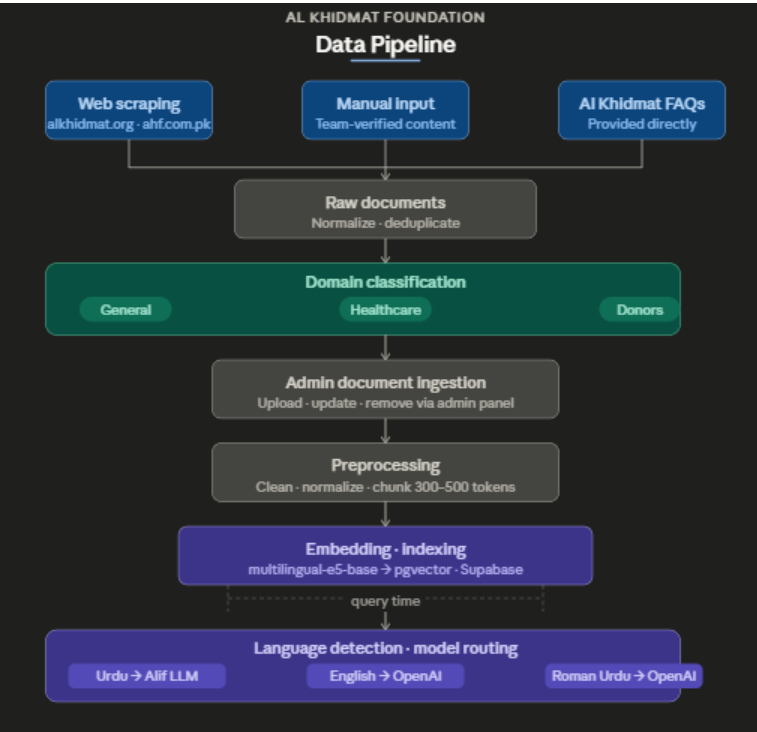
\includegraphics[width=0.8\textwidth]{chapters/data_pipeline.png}
    \caption{Data Pipeline Architecture}
    \label{fig:data-pipeline}
\end{figure}

% % This appendix is required if the code is not fully described in the main text.
% \chapter{Code}
% \input{chapters/appendix-code}
% \end{appendices}

% Print the bibliography using biblatex and include it in the TOC.
\clearpage
\printbibliography[heading=bibintoc,title=References]

\end{document}

%%% Local Variables:
%%% mode: latex
%%% TeX-master: t
%%% End:
